% Copyright (c) 2015 Daniele Masini - d.masini.it@gmail.com
% Copyright (c) 2016 Daniele Zambelli - daniele.zambelli@gmail.com

\chapter{Equiestensione e aree}\label{chap:equiestensione_aree}

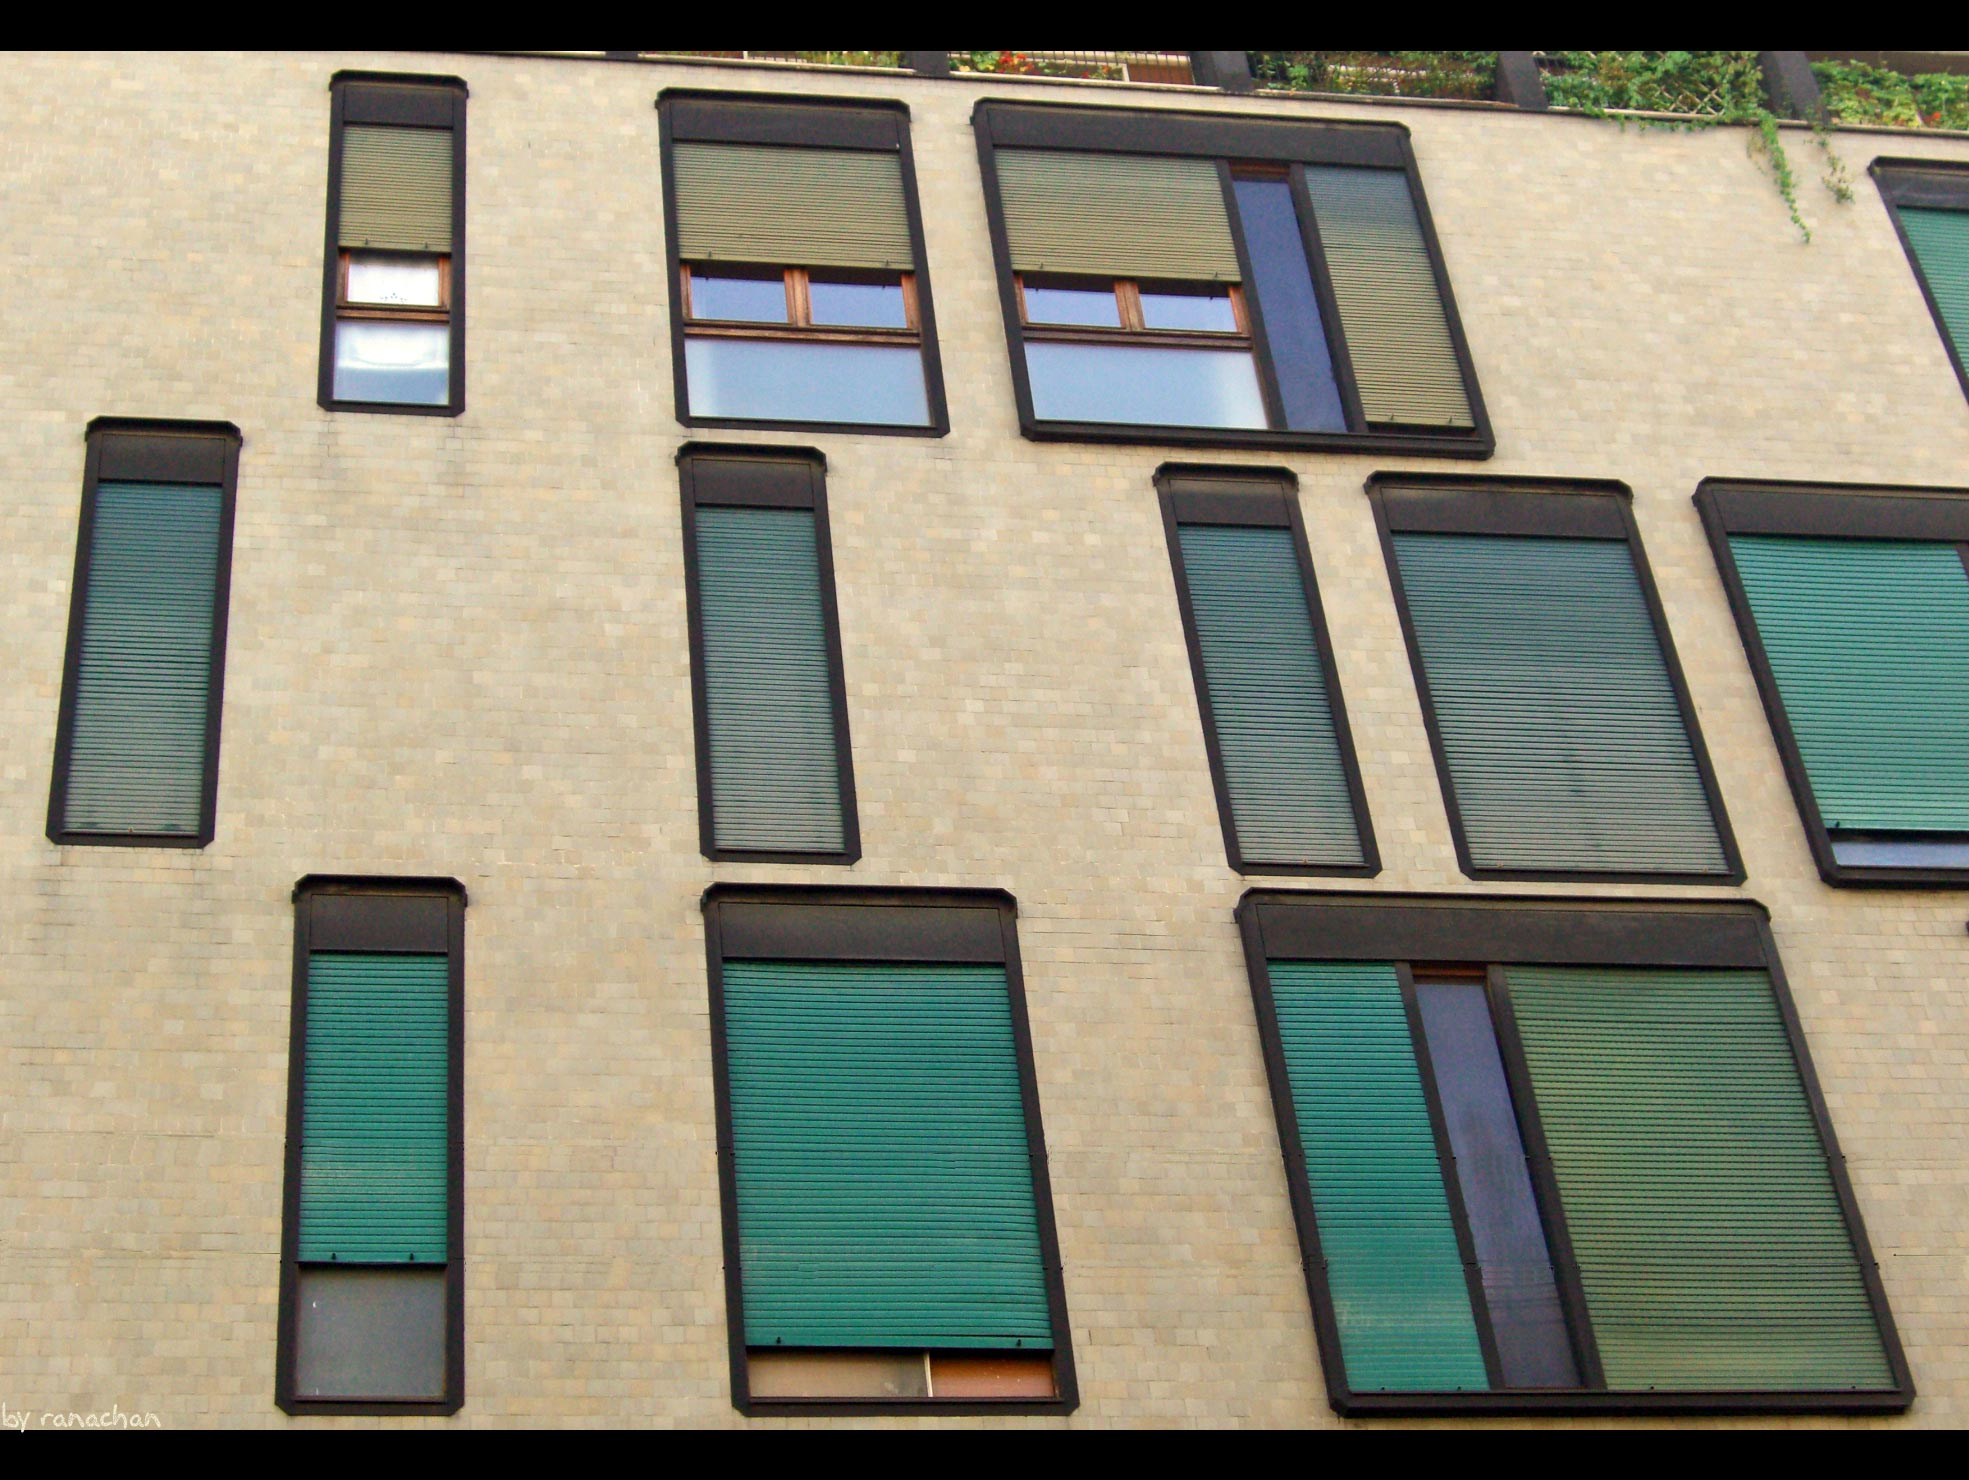
\includegraphics[width=0.95\textwidth]{\folder img/window_geometry.jpg}
  \begin{center}
    {\large ``Window geometry''}\par
    Foto di midori.no.kerochan\par
    \url{http://www.flickr.com/photos/28661972@N05/2751042868/}\par
    Licenza: Creative Commons Attribution 2.0\par
  \end{center}
\newpage


\section{Estensione superficiale}\label{sect:estensione_superficiale}

Il \emph{tangram}\label{tangram} è un antichissimo gioco cinese. Il 
nome con cui lo conosciamo si pensa derivato dall'unione della parola 
\emph{tang} o \emph{tan}, che significa \emph{cinese}, e \emph{gram} 
che significa \emph{immagine}. Anticamente in Cina era chiamato 
``schema intelligente a sette pezzi'' o anche ``le sette pietre della 
saggezza'' poiché si riteneva che la padronanza del gioco fosse la 
chiave per ottenere saggezza e talento.
Il gioco è costituito da un quadrato ritagliato in 7~pezzi poligonali 
aventi in comune solo punti del loro contorno 
(figura~\ref{fig:tangram}).


\begin{inaccessibleblock}[Figura: TODO]
 \begin{figure}[!htb]
  \centering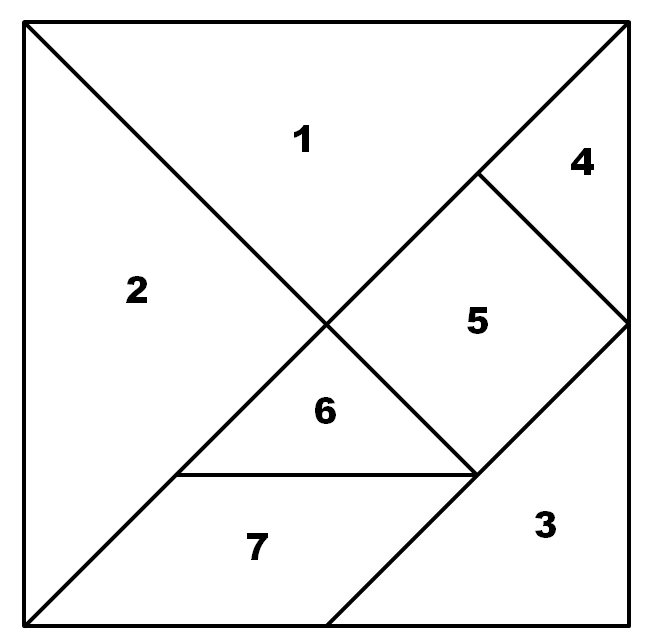
\includegraphics[width=0.6\textwidth]{\folder img/tangram.png}
  \caption{Il gioco del tangram}\label{fig:tangram}
\end{figure}
\end{inaccessibleblock}

I pezzi possono essere disposti e accostati gli uni agli altri senza 
sovrapposizioni in modo da ottenere una grande varietà di figure; la 
regola base è che devono essere utilizzati tutti i 7~pezzi. Si 
possono così formare alcuni disegni come mostrato nella 
figura~\ref{fig:figure_tangram}.


\begin{inaccessibleblock}[Figura: TODO]
 \begin{figure}[!htb]
 \centering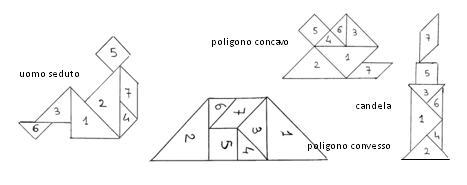
\includegraphics[width=0.8\textwidth]
    {\folder img/figure_tangram.png}
  \caption{Alcune figure realizzabili con il 
tangram}\label{fig:figure_tangram}
\end{figure}
\end{inaccessibleblock}

Potete osservare che si forma un poligono quando i singoli pezzi 
vengono accostati mediante un lato: l'uomo seduto è un poligono, ma 
non la candela; i due poligoni rappresentati sono l'uno concavo e 
l'altro convesso.

Con tutti i 7~pezzi del gioco si possono costruire 13~poligoni 
convessi, compreso il quadrato iniziale, provate a costruirli: 
fotocopiate la pagina precedente e ritagliate i 7~pezzi del tangram.

Evidentemente i 13~poligoni che avrete costruito non sono congruenti, 
né hanno la stessa forma; potete dire che sono formati dalle stesse 
parti poligonali, ciascuno può cioè essere pensato come unione dei 
\emph{tan} aventi in comune almeno un punto del loro perimetro, ma 
nessun punto interno.

\begin{definizione}
Con \emph{somma} di due \emph{figure piane} \(X\) e \(Y\), non aventi 
punti comuni o aventi in comune solo punti del loro contorno, 
intendiamo la figura \(Z\) unione dei punti di \(X\) e \(Y\) e la 
indicheremo con
\[\boxed{Z=X+Y}\]
Diremo inoltre che \(X\) è la \emph{differenza} tra \(Z\) e \(Y\) e 
scriveremo
\[\boxed{X=Z-Y}\]
\end{definizione}

\begin{definizione}
Due poligoni \(p_1\) e \(p_2\) sono \emph{equicomposti} se sono formati 
dalle stesse parti poligonali (figure piane). Sono 
\emph{equiscomponibili} se è possibile decomporre uno di essi in un 
numero finito di parti poligonali con le quali si possa ricoprire 
l'altro. In simboli
\[\boxed{\vphantom{I}p_1 \doteq p_2}\]
\noindent che si legge ``\(p_1\) equicomposto \(p_2\)''
\end{definizione}

Tutte le figure poligonali costruite con i pezzi del tangram \(p_1\), 
\(p_2\), \ldots{} sono dunque poligoni equicomposti, ma possono anche 
essere considerati poligoni equiscomponibili, quindi \(p_1 \doteq p_2 
\doteq \ldots{}\)

\begin{exrig}
\noindent\begin{minipage}{0.65\textwidth}\parindent15pt
\begin{esempio}\label{es:7.1}
Ritagliate da un quadrato i quattro triangoli rettangoli isosceli che 
si ottengono tracciando le sue diagonali (fotocopia e ritaglia la 
figura a fianco). Disponendo fianco a fianco i triangoli ottenuti in 
modo che i due lati comuni abbiano la stessa lunghezza, si ottengono 
14~figure diverse. Due di esse sono riportate nella 
figura~\ref{fig:quadrato2}. Realizzate tutte le altre figure.
\end{esempio}
\end{minipage}\hfil
\begin{minipage}{0.35\textwidth}
	\centering% Copyright (c) 2015 Daniele Masini - d.masini.it@gmail.com

\begin{tikzpicture}[scale=1.2,font=\small]
\usetikzlibrary{calc}

\begin{scope}

\draw (0,0) -- (2,2);
\draw (0,2) -- (2,0);
\draw (0,0) -- (2,0) -- (2,2) -- (0,2) -- cycle;

\node at (0.4,1) {1};
\node at (1,1.6) {2};
\node at (1.6,1) {3};
\node at (1,0.4) {4};

\end{scope}

\end{tikzpicture}

\end{minipage}\vspace{5pt}


\begin{inaccessibleblock}[Figura: TODO]
 \begin{figure}[!htb]
\centering% Copyright (c) 2015 Daniele Masini - d.masini.it@gmail.com

\begin{tikzpicture}[scale=1.2,font=\small]
\usetikzlibrary{calc}

\begin{scope}

\draw (0,0) -- (4,0);
\draw (1,1) -- (5,1);
\draw (0,0) -- (1,1) -- (2,0) -- (3,1) -- (4,0) -- (5,1);

\end{scope}


\begin{scope}[xshift=6cm, yshift=0.5cm]

\draw (0,0) -- (2,0);
\draw (1,1) -- (3,1);
\draw (0,0) -- (1,1) -- (2,0) -- (3,1) -- (3,-1) -- (2,0) -- (1,-1) -- (3,-1);

\end{scope}

\end{tikzpicture}

\caption{Alcune figure realizzabili 
(esempio~\ref{es:7.1})}\label{fig:quadrato2}
\end{figure}
\end{inaccessibleblock}

Le figure ottenute sono \ldots\ldots\ldots\ldots{} perché sono 
formate da \ldots\ldots\ldots\ldots{}

\noindent(da: Prova di allenamento della gara di ``Matematica senza 
frontiere'' del 9/02/1994)

\begin{esempio}\label{es:7.2}
Nella figura~\ref{fig:figure} sono disegnati un quadrato \(ABCD\), un 
rettangolo \(PQRS\) avente \(PQ=2AB\) e \(SP=AB/2\) e un rombo \(FGHK\) 
avente una diagonale uguale al lato del quadrato e l'altra il doppio. 
Mostra come sia possibile scomporre ciascuno dei tre poligoni in parti 
tali da poter ricoprire gli altri due. Puoi concludere che i tre 
poligoni assegnati sono equiscomponibili? \ldots\ldots{}


\begin{inaccessibleblock}[Figura: TODO]
 \begin{figure}[!htb]
	\centering% Copyright (c) 2015 Daniele Masini - d.masini.it@gmail.com

\begin{tikzpicture}[scale=1.5,font=\small]
\usetikzlibrary{calc}

\begin{scope}
\draw (0,0) rectangle (1,1);
\node[shift={(-.2,-.2)}] at (0,0) {$A$};
\node[shift={(.2,-.2)}] at (1,0) {$D$};
\node[shift={(.2,.2)}] at (1,1) {$C$};
\node[shift={(-.2,.2)}] at (0,1) {$D$};
\end{scope}

\begin{scope}[xshift=2cm, yshift=0.25cm]
\draw (0,0) rectangle (2,0.5);
\node[shift={(-.2,-.2)}] at (0,0) {$P$};
\node[shift={(.2,-.2)}] at (2,0) {$Q$};
\node[shift={(.2,.2)}] at (2,0.5) {$R$};
\node[shift={(-.2,.2)}] at (0,0.5) {$S$};
\end{scope}

\begin{scope}[xshift=5cm, yshift=0.5cm]
\draw (0,0) node[shift={(-.2,0)}] {$F$} -- (1,-0.5) node[shift={(0,-.2)}] {$G$} -- (2,0) node[shift={(.2,0)}] {$H$} -- (1,0.5) node[shift={(0,.2)}] {$K$} -- cycle;
\end{scope}

\end{tikzpicture}

	\caption{Esempio~\ref{es:7.2}}\label{fig:figure}
\end{figure}
\end{inaccessibleblock}

\end{esempio}

\noindent\begin{minipage}{0.6\textwidth}\parindent15pt
\begin{esempio}\label{es:7.3}
Dato l'insieme \(F = \{f_1\text{,}f_2\text{,}f_3\}\) delle figure 
poligonali disegnate a lato, segui le seguenti istruzioni:\\
\verb|   |\textsl{ripeti:}\\
\verb|      |\textsl{scegli una figura dell'insieme \(F\);}\\
\verb|      |\textsl{traccia alcuni segmenti che la decompongano in}\\
\verb|        |\textsl{parti poligonali;}\\
\verb|      |\textsl{forma con le parti ottenute altre 3 figure 
poligo-}\\
\verb|        |\textsl{nali;}\\
\verb|   |\textsl{finché non hai esaurito le figure.}\\
Costruisci l'insieme \(G\) di tutti i poligoni ottenuti con questa 
procedura e indica con simboli arbitrari i suoi elementi.
\end{esempio}
\end{minipage}\hfil
\begin{minipage}{0.4\textwidth}
	\centering% Copyright (c) 2015 Daniele Masini - d.masini.it@gmail.com

\begin{tikzpicture}[scale=2,font=\small]
\usetikzlibrary{calc}

\begin{scope}
\draw (0,0) -- (1,0) -- (0.75,0.5) -- (-0.25,0.5) -- cycle;
\node at (0.4,0.25) {$f_1$};
\end{scope}

\begin{scope}[xshift=1.7cm]
\draw (0,0) -- (0.5,0.5) -- (-0.4,0.5) -- cycle;
\node at (0,0.3) {$f_2$};
\end{scope}

\begin{scope}[xshift=0.25cm, yshift=-1.1cm]
\draw (0,0) -- (1.5,0) -- (1,0.7) -- (0.25,0.5) -- cycle;
\node at (0.7,0.25) {$f_3$};
\end{scope}

\end{tikzpicture}

\end{minipage}\vspace{5pt}

\end{exrig}

Nell'insieme \(S=F\cup G\) (dove \(F\) e \(G\) sono gli insiemi definiti 
nell'esempio~\ref{es:7.3}) la relazione \(R\) espressa dal predicato: 
<<essere equicomposti>> gode della proprietà
\begin{itemize*}
\item riflessiva, infatti \ldots\ldots\ldots\ldots\ldots{}
\item simmetrica, infatti \ldots\ldots\ldots\ldots\ldots{}
\item transitiva, infatti \ldots\ldots\ldots\ldots\ldots{}
\end{itemize*}
Si può dunque concludere che \(R\) è una relazione di equivalenza e 
quindi si possono costruire sia l'insieme delle parti \(P(S)\), sia 
l'insieme quoziente \(E=S/R\) avente come elementi le tre classi di 
equivalenza, ciascuna rappresentata dal poligono iniziale 
(figura~\ref{fig:insiemi}):
\[ [f_1] = \{x:x\text{ è un poligono equicomposto con }f_1\}; \]
\[ [f_2] = \{x:x\text{ è un poligono equicomposto con }f_2\}; \]
\[ [f_3] = \{x:x\text{ è un poligono equicomposto con }f_3\}. \]


\begin{inaccessibleblock}[Figura: TODO]
 \begin{figure}[!htb]
	\centering% Copyright (c) 2015 Daniele Masini - d.masini.it@gmail.com

\begin{tikzpicture}[scale=0.8,font=\small]
\usetikzlibrary{calc}

\begin{scope}
\draw (0,0) circle (2);
\draw[fill] (90:1.8) circle (1pt);
\draw[fill] (120:1.25) circle (1pt)  node[above] {$f_1$};
\draw[fill] (150:1.5) circle (1pt);
\draw[fill] (180:1.8) circle (1pt);
\draw (70:2) -- (190:2);
\draw[fill] (80:0.5) circle (1pt);
\draw[fill] (180:1) circle (1pt);
\draw[fill] (210:1.5) circle (1pt);
\draw[fill] (250:1.3) circle (1pt) node[above] {$f_2$};
\draw (70:2) -- (270:2);
\draw[fill] (300:1.2) circle (1pt);
\draw[fill] (330:1.3) circle (1pt);
\draw[fill] (40:1) circle (1pt);
\draw[fill] (10:1.5) circle (1pt) node[above] {$f_3$};
\node at (0,-2.5) {$P(S)$};
\end{scope}

\begin{scope}[xshift=5cm]
\draw (0,0) circle (2);
\draw[fill] (120:1) circle (1pt) node[above] {$[f_1]$};
\draw[fill] (250:1.3) circle (1pt) node[above] {$[f_2]$};
\draw[fill] (340:0.9) circle (1pt) node[above] {$[f_3]$};
\node at (0,-2.5) {$E$};
\end{scope}

\end{tikzpicture}

	\caption{Rappresentazione dell'insieme delle parti di \(S\) e 
del quoziente \(E=S/R\)}\label{fig:insiemi}
\end{figure}
\end{inaccessibleblock}

\begin{definizione}
Diciamo che due qualunque poligoni \(p_1\) e \(p_2\) appartenenti alla 
stessa classe sono \emph{equivalenti} e useremo la scrittura 
\(p_1\doteq p_2\) per esprimere questa caratteristica 
(\emph{equivalenza per scomposizione}); essi hanno una caratteristica 
comune che chiamiamo \emph{estensione superficiale} (ES).
\end{definizione}

I poligoni costruiti con i pezzi del tangram appartengono alla stessa 
classe di equivalenza; essi sono dunque poligoni equivalenti e hanno 
la stessa estensione superficiale del quadrato iniziale.
Anche i 14~poligoni realizzati nell'esempio~\ref{es:7.1} appartengono 
alla stessa classe di equivalenza; essi sono dunque poligoni 
equivalenti e hanno la stessa estensione superficiale del quadrato 
assegnato.

\osservazione Sin dalla scuola elementare avete usato termini come 
``superficie'', ``estensione'' e ``area'' quando vi siete accostati 
allo studio dei poligoni, probabilmente ritenendoli sinonimi. Lo 
studio di una particolare relazione di equivalenza vi ha mostrato che 
il concetto di estensione di un poligono si ottiene attraverso il 
procedimento di passaggio al quoziente nell'insieme dei poligoni 
piani.

\begin{definizione}
Chiamiamo \emph{area} di un poligono \(p\) il numero reale positivo 
\(A(p)\) che esprime la misura della sua estensione superficiale.
\end{definizione}

Possiamo concludere che ad ogni classe di equivalenza, generata con 
la relazione <<essere equicomposti>> o <<essere equiscomponibili>>, 
può essere associato un numero: l'area della figura scelta come 
rappresentante della classe di equivalenza. In tal modo trasformeremo 
una relazione di equivalenza tra poligoni, espressa con il simbolo 
\(\doteq\) in una relazione di uguaglianza tra numeri.
Ad esempio, riferendoci ai poligoni costruiti con i pezzi del tangram 
possiamo trasformare la relazione di equivalenza \(p_1\doteq p_2\doteq 
p_3\doteq \ldots{}\) in un'uguaglianza tra le aree scrivendo 
\(A(p_1)=A(p_2)=A(p_3)=\ldots{}\)

\section{Poligoni equivalenti}\label{sect:poligoni_equivalenti}

Premettiamo alcuni assiomi:
\nopagebreak
\begin{enumerate}
\item Poligoni congruenti sono equivalenti.
\item Un poligono non è equivalente ad una sua parte propria.
\item Somma e differenza di poligoni equivalenti originano poligoni 
equivalenti.
\end{enumerate}

\begin{teorema}\label{teo:7.1}
Due parallelogrammi aventi rispettivamente congruenti le basi e le 
rispettive altezze, sono equivalenti.
\end{teorema}

Nella figura sottostante sono rappresentati alcuni degli infiniti 
parallelogrammi aventi basi e altezze congruenti; le loro basi 
appartengono a rette parallele.

\noindent Ipotesi: \(AB\cong EF\cong IJ\), \(DM\perp AB\), \(HN\perp EF\), 
\(LO\perp IJ\), \(DM\cong HN\cong LO\).\\
Tesi: \(ABCD\doteq EFGH\doteq IJLK\).\\

\begin{figure*}[!htb]
	
\centering% Copyright (c) 2015 Daniele Masini - d.masini.it@gmail.com

\begin{tikzpicture}[scale=1.2,font=\small]
\usetikzlibrary{calc}

\draw[dotted] (-0.5,0) -- (9,0);
\draw[dotted] (-0.5,1.5) -- (9,1.5);
\begin{scope}
\draw[thick, fill=red!10] (0,0) coordinate (a) node[shift={(-0.2,-0.2)}] {$A$} -- (1,0) coordinate (b) node[shift={(0.2,-0.2)}] {$B$} -- (1.3,1.5) coordinate (c) node[shift={(0.2,0.2)}] {$C$} -- (0.3,1.5) coordinate (d) node[shift={(-0.2,0.2)}] {$D$} -- cycle;
\draw[dashed, red] (d) -- ($(a)!(d)!(b)$) node[below, black] {$M$};
\draw[thick, blue] (a) -- (b);
\end{scope}

\begin{scope}[xshift=2.2cm]
\draw[thick, fill=red!10] (0,0) coordinate (e) node[shift={(-0.2,-0.2)}] {$E$} -- (1,0) coordinate (f) node[shift={(0.2,-0.2)}] {$F$} -- (2.4,1.5) coordinate (g) node[shift={(0.2,0.2)}] {$G$} -- (1.4,1.5) coordinate (h) node[shift={(-0.2,0.2)}] {$H$} -- cycle;
\draw[dashed, red] (h) -- ($(e)!(h)!(f)$) node[below, black] {$N$};
\draw[thick, blue] (e) -- (f);
\end{scope}

\begin{scope}[xshift=5cm]
\draw[thick, fill=red!10] (0,0) coordinate (i) node[shift={(-0.2,-0.2)}] {$I$} -- (1,0) coordinate (j) node[shift={(0.2,-0.2)}] {$J$} -- (3.4,1.5) coordinate (k) node[shift={(0.2,0.2)}] {$K$} -- (2.4,1.5) coordinate (l) node[shift={(-0.2,0.2)}] {$L$} -- cycle;
\draw[dashed, red] (l) -- ($(i)!(l)!(j)$) node[below, black] {$O$};
\draw[thick, blue] (i) -- (j);
\end{scope}

\end{tikzpicture}

\end{figure*}

\begin{proof}
Per dimostrare l'equivalenza tra questi parallelogrammi, costruiamo 
su \(ABCD\) un altro parallelogramma, facendo sovrapporre le loro basi. 
Avremo tre casi:\\

\noindent\begin{minipage}{0.75\textwidth}\parindent15pt
\noindent\emph{Primo caso}\\
Costruiamo su \(ABCD\) il parallelogramma \(ABC'D'\) avente la stessa 
base \(AB\) e la stessa altezza; il vertice \(D'\) è un punto interno a 
\(DC\). \(ABCD\) è scomposto in \(ADD' + ABCD'\); \(ABC'D'\) è scomposto in 
\(BCC' + ABCD'\). Se dimostriamo la congruenza dei triangoli \(ADD'\) e 
\(BCC'\) potremo concludere che i due parallelogrammi, essendo 
equicomposti, sono equivalenti.
Consideriamo i due triangoli \(ADD'\) e \(BCC'\), essi sono congruenti 
per il terzo criterio di congruenza, infatti: \(AD\cong BC\) perché 
lati opposti del parallelogramma \(ABCD\); \(AD'\cong BC'\) perché lati 
opposti del parallelogramma \(ABC'D'\); \(DD'\cong CC'\) perché differenza 
di segmenti congruenti, precisamente \(DD'=DC-D'C\) e \(CC'=C'D'-CD'\). 
Dalla congruenza dei triangoli segue anche la loro equivalenza 
\(ADD'\cong BCC' \:\Rightarrow\: ADD'\doteq BCC'\). Possiamo allora 
concludere che \(ABCD\doteq ABC'D'\).\\
\end{minipage}\hfil
\begin{minipage}{0.25\textwidth}
	
\centering% Copyright (c) 2015 Daniele Masini - d.masini.it@gmail.com

\begin{tikzpicture}[scale=1.2,font=\small]
\usetikzlibrary{calc}

\begin{scope}
\path[fill=blue!10, opacity=0.4] (0,0) coordinate (a) -- (1,0) coordinate (b) -- (1.3,2) coordinate (c) -- (0.3,2) coordinate (d) -- cycle;
\path[fill=red!10, opacity=0.4] (a) -- (b) -- (1.7,2) coordinate (c1) -- (0.7,2) coordinate (d1) -- cycle;
\draw[thick] (a) node[shift={(-0.2,-0.2)}] {$A$} -- (b) node[shift={(0.2,-0.2)}] {$B$} -- (c) node[shift={(0.2,0.2)}] {$C$} -- (d) node[shift={(-0.2,0.2)}] {$D$} -- cycle;
\draw[thick] (a) -- (b) -- (c1) node[shift={(0.2,0.2)}] {$C'$} -- (d1) node[shift={(-0.2,0.2)}] {$D'$} -- cycle;
\end{scope}

\end{tikzpicture}

\end{minipage}
\noindent\begin{minipage}{0.7\textwidth}\parindent15pt
\noindent\emph{Secondo caso}\\
Costruiamo su \(ABCD\) il parallelogramma \(ABC'D'\) avente la stessa 
base \(AB\) e la stessa altezza; il vertice \(C\) coincide con \(D'\) e 
\(ABCD\) è scomposto in \(ADC + ACB\); \(ABC'D'\) è scomposto in \(ABD' + 
BC'D'\). Se dimostriamo la congruenza dei triangoli \(ADC\) e \(BC'D'\) 
possiamo concludere che i due parallelogrammi, essendo equicomposti, 
sono equivalenti. Infatti, \(ADC\) e \(BC'D'\) hanno \(AD\cong CB\) perché 
lati opposti di uno stesso parallelogramma, \(DC\cong C'D'\), \(AC\cong 
BC'\), pertanto \(ADC\) e \(BC'D'\) sono triangoli congruenti.\\
\end{minipage}\hfil
\begin{minipage}{0.3\textwidth}
	
\centering% Copyright (c) 2015 Daniele Masini - d.masini.it@gmail.com

\begin{tikzpicture}[scale=1.2,font=\small]
\usetikzlibrary{calc}

\begin{scope}
\path[fill=blue!10, opacity=0.4] (0,0) coordinate (a) -- (1,0) coordinate (b) -- (1.3,2) coordinate (c) -- (0.3,2) coordinate (d) -- cycle;
\path[fill=red!10, opacity=0.4] (a) -- (b) -- (2.3,2) coordinate (c1) -- (c) -- cycle;
\draw[thick] (a) node[shift={(-0.2,-0.2)}] {$A$} -- (b) node[shift={(0.2,-0.2)}] {$B$} -- (c) node[shift={(0,0.2)}] {$C\equiv D'$} -- (d) node[shift={(-0.2,0.2)}] {$D$} -- cycle;
\draw[thick] (a) -- (b) -- (c1) node[shift={(0.2,0.2)}] {$C'$} -- (c) -- cycle;
\end{scope}

\end{tikzpicture}

\end{minipage}
\noindent\begin{minipage}{0.65\textwidth}\parindent15pt
\noindent\emph{Terzo caso}\\
Costruiamo su \(ABCD\) il parallelogramma \(ABC'D'\) avente la stessa 
base \(AB\) e la stessa altezza; il vertice \(D'\) è esterno al lato \(DC\) 
e i lati \(AD'\) e \(BC\) si intersecano nel punto \(G\).
\(ABCD\) è scomposto in \(ADCG + AGB\) mentre \(ABC'D'\) è scomposto in 
\(BGD'C' + AGB\), inoltre \(ADCG\) si può scomporre in \(ADD' - CGD'\) come 
\(BGD'C'\) si può scomporre in \(BCC' - CGD'\).
Quindi \(ABCD\) è scomposto in \(ADD' - CGD' + AGB\) e \(ABC'D'\) è 
scomposto in \(BCC' - CGD' + AGB\).
Basta allora dimostrare la congruenza dei triangoli \(ADD'\) e \(BCC'\) 
per dire che \(ABCD\) e \(ABC'D'\) sono equiscomposti e dunque 
equivalenti. Infatti \(ADD'\) e \(BCC'\) sono congruenti perché hanno 
\(AD\cong BC\), lati opposti del parallelogramma, analogamente 
\(AD'\cong BC'\) e \(DD'\cong CC'\) perché somma di segmenti congruenti.
\end{minipage}\hfil
\begin{minipage}{0.35\textwidth}
	
\centering% Copyright (c) 2015 Daniele Masini - d.masini.it@gmail.com

\begin{tikzpicture}[scale=1.2,font=\small]
\usetikzlibrary{calc}

\begin{scope}
\path[fill=blue!10, opacity=0.4] (0,0) coordinate (a) -- (1,0) coordinate (b) -- (1.3,2) coordinate (c) -- (0.3,2) coordinate (d) -- cycle;
\path[fill=red!10, opacity=0.4] (a) -- (b) -- (3,2) coordinate (c1) -- (2,2) coordinate (d1) -- cycle;
\draw[thick] (a) -- (b) -- (c1) node[shift={(0.2,0.2)}] {$C'$} -- (d1) node[shift={(-0.2,0.2)}] {$D'$} -- cycle;
\draw[thick] (a) node[shift={(-0.2,-0.2)}] {$A$} -- (b) node[shift={(0.2,-0.2)}] {$B$} -- (c) node[shift={(0.2,0.2)}] {$C$} -- (d) node[shift={(-0.2,0.2)}] {$D$} -- cycle;

\draw[fill] (intersection of d1--a and c--b) circle (1pt) node[right] {$G$};
\draw[dotted] (c)-- (d1);
\end{scope}

\end{tikzpicture}

\end{minipage}
\end{proof}

\begin{corollario}\label{cor:7.1}
Ogni parallelogramma è equivalente al rettangolo avente un lato 
congruente alla sua base e l'altro lato congruente alla sua altezza.
\end{corollario}

\noindent Ipotesi: \(AB\cong EF\), \(CF\perp AB\), \(CK\cong HE\).\\
Tesi: \(ABCD\doteq EFGH\).

\begin{figure*}[!htb]
	\centering% Copyright (c) 2015 Daniele Masini - d.masini.it@gmail.com

\begin{tikzpicture}[scale=1.2,font=\small]
\usetikzlibrary{calc}

\begin{scope}
\draw[thick, fill=red!10] (0,0) coordinate (a) node[shift={(-0.2,-0.2)}] {$A$} -- (2,0) coordinate (b) node[shift={(0.2,-0.2)}] {$B$} -- (1.5,1.5) coordinate (c) node[shift={(0.2,0.2)}] {$C$} -- (-0.5,1.5) coordinate (d) node[shift={(-0.2,0.2)}] {$D$} -- cycle;
\draw[dashed, red] (c) -- ($(a)!(c)!(b)$) node[below, black] {$K$};
\draw[thick, blue] (a) -- (b);
\end{scope}

\begin{scope}[xshift=3.5cm]
\draw[thick, fill=red!10] (0,0) coordinate (e) node[shift={(-0.2,-0.2)}] {$E$} -- (2,0) coordinate (f) node[shift={(0.2,-0.2)}] {$F$} -- (2,1.5) coordinate (g) node[shift={(0.2,0.2)}] {$G$} -- (0,1.5) coordinate (h) node[shift={(-0.2,0.2)}] {$H$} -- cycle;
\draw[thick, red] (e) -- (h);
\draw[thick, blue] (e) -- (f);
\end{scope}

\end{tikzpicture}

\end{figure*}

\noindent\begin{minipage}{0.65\textwidth}\parindent15pt
\begin{proof}
Dal vertice \(D\) tracciamo l'altezza \(DL\) relativa alla base \(AB\); il 
quadrilatero \(DLKC\) è un rettangolo congruente a \(EFGH\); dimostrando 
che \(ABCD\doteq DLKC\) si ottiene la tesi.\\
Completate la dimostrazione.\\
Osserviamo che \(ABCD\) è composto da \ldots\ldots\ldots\ldots{}
e \(DLKC\) è composto da \ldots\ldots\ldots\ldots{} 
Consideriamo i triangoli \ldots\ldots\ldots\ldots{}
Sono congruenti perché \ldots\ldots\ldots\ldots{}
quindi \ldots\ldots\ldots\ldots{}
\end{proof}
\end{minipage}\hfil
\begin{minipage}{0.35\textwidth}
	\centering% Copyright (c) 2015 Daniele Masini - d.masini.it@gmail.com

\begin{tikzpicture}[scale=1.2,font=\small]
\usetikzlibrary{calc}

\begin{scope}
\path[fill=red!10, opacity=0.5] (0,0) coordinate (a) -- (2,0) coordinate (b) -- (1.5,1.5) coordinate (c) -- (-0.5,1.5) coordinate (d) -- cycle;
\draw[thick] (a) node[shift={(-0.2,-0.2)}] {$A$} -- (b) node[shift={(0.2,-0.2)}] {$B$} -- (c) node[shift={(0.2,0.2)}] {$C$} -- (d) node[shift={(-0.2,0.2)}] {$D$} -- cycle;
\node[below] at ($(a)!(c)!(b)$) {$K$};
\end{scope}

\begin{scope}[xshift=-.5cm]
\path[fill=red!10, opacity=0.5] (0,0) coordinate (e) -- (2,0) coordinate (f) -- (2,1.5) coordinate (g) -- (0,1.5) coordinate (h) -- cycle;
\draw[thick] (e) node[shift={(-0.2,-0.2)}] {$L$} -- (f) -- (g) -- (h) -- cycle;
\end{scope}

\end{tikzpicture}

\end{minipage}\vspace{5pt}

Il teorema~\ref{teo:7.1} e il suo corollario~\ref{cor:7.1} ci 
assicurano che i parallelogrammi aventi rispettivamente congruenti le 
basi e le relative altezze formano una classe di equivalenza avente 
come rappresentante il rettangolo che ha un lato congruente alla base 
del parallelogramma e l'altro lato congruente alla sua altezza. 
Possiamo quindi affermare che \(ABCD\doteq EFGH \:\Rightarrow\: 
A_{ABCD} = A_{EFGH}\).

\begin{teorema}\label{teo:7.2}
Un triangolo è equivalente ad un parallelogramma avente:
\begin{enumeratea}
\item base congruente alla metà della base del triangolo e altezza 
congruente all'altezza del triangolo, oppure
\item base congruente alla base del triangolo e altezza congruente 
alla metà dell'altezza del triangolo.
\end{enumeratea}
\end{teorema}

Nella figura sono rappresentati il triangolo \(ABC\), il 
parallelogramma \(DEFG\) avente base congruente alla metà della base del 
triangolo e altezza congruente all'altezza del triangolo, il 
parallelogramma \(IJLM\) avente altezza congruente alla metà 
dell'altezza del triangolo e base congruente alla base del triangolo.

\noindent Ipotesi: \(AB\perp CH\), \(DE\cong \frac{1}{2}AB\), \(GK\perp 
DE\), \(GK\cong CH\), \(IJ\cong AB\), \(MN\perp IJ\), \(MN\cong 
\frac{1}{2}CH\).\\
Tesi: a) \(ABC\doteq DEFG\);\quad b) \(ABC\doteq IJLM\).

\begin{figure*}[!htb]
	\centering% Copyright (c) 2015 Daniele Masini - d.masini.it@gmail.com

\begin{tikzpicture}[scale=1.2,font=\small]
\usetikzlibrary{calc}

\begin{scope}
\draw[thick, fill=red!10] (0,0) coordinate (a) node[shift={(-0.2,-0.2)}] {$A$} -- (2,0) coordinate (b) node[shift={(0.2,-0.2)}] {$B$} -- (0.5,1.5) coordinate (c) node[shift={(0,0.2)}] {$C$} -- cycle;
\draw[dashed, red] (c) -- ($(a)!(c)!(b)$) node[below, black] {$H$};
\draw[thick, blue] (a) -- (b);
\end{scope}

\begin{scope}[xshift=3.5cm]
\draw[thick, fill=red!10] (0,0) coordinate (d) node[shift={(-0.2,-0.2)}] {$D$} -- (1,0) coordinate (e) node[shift={(0.2,-0.2)}] {$E$} -- (1.3,1.5) coordinate (f) node[shift={(0.2,0.2)}] {$F$} -- (0.3,1.5) coordinate (g) node[shift={(-0.2,0.2)}] {$G$} -- cycle;
\draw[dashed, red] (g) -- ($(d)!(g)!(e)$) node[below, black] {$K$};
\draw[thick, green!80!black] (d) -- (e);
\end{scope}

\begin{scope}[xshift=6cm]
\draw[thick, fill=red!10] (0,0) coordinate (i) node[shift={(-0.2,-0.2)}] {$I$} -- (2,0) coordinate (j) node[shift={(0.2,-0.2)}] {$J$} -- (2.3,0.75) coordinate (l) node[shift={(0.2,0.2)}] {$L$} -- (0.3,0.75) coordinate (m) node[shift={(-0.2,0.2)}] {$M$} -- cycle;
\draw[dashed, orange!70!black] (m) -- ($(i)!(m)!(j)$) node[below, black] {$N$};
\draw[thick, blue] (i) -- (j);
\end{scope}

\end{tikzpicture}

\end{figure*}

\begin{proof}~\vspace{4pt}\\
\noindent\begin{minipage}{0.65\textwidth}\parindent15pt
\noindent\emph{Caso a.}\\
Dal punto medio \(T\) della base \(AB\) tracciamo la parallela al lato 
\(AC\) che incontra \(CB\) in \(S\); dal vertice \(C\) tracciamo la 
parallela 
alla base \(AB\) che interseca in \(R\) la retta \(ST\); il parallelogramma 
\(ATRC\) soddisfa le ipotesi del caso a) ed è equivalente a \(DEFG\) per 
il teorema~\ref{teo:7.1}.
Confrontiamo il triangolo e il parallelogramma: possiamo pensare 
\(ABC\) composto da \(CATS+BST\) e \(ATRC\) composto da \(CATS+CSR\).
Se dimostriamo la congruenza dei triangoli \(CSR\) e \(BST\) potremo 
concludere che triangolo e parallelogramma, essendo equicomposti, 
sono equivalenti. 
\(TB\cong CR\) infatti \ldots\ldots\ldots\ldots{}
\(SB\cong CS\) infatti \ldots\ldots\ldots\ldots{}
\(T\widehat{B}S\cong S\widehat{C}R\) infatti \ldots\ldots\ldots\ldots{}
Allora per il primo criterio di congruenza \(TBS\cong SCR\) e quindi 
\(ATRC\doteq BST\).\\
\end{minipage}\hfil
\begin{minipage}{0.35\textwidth}
	\centering% Copyright (c) 2015 Daniele Masini - d.masini.it@gmail.com

\begin{tikzpicture}[scale=1.2,font=\small]
\usetikzlibrary{calc}

\begin{scope}
\draw[thick, fill=red!10] (0,0) coordinate (a) node[shift={(-0.2,-0.2)}] {$A$} -- (2,0) coordinate (b) node[shift={(0.2,-0.2)}] {$B$} -- (0.5,1.5) coordinate (c) node[shift={(0,0.2)}] {$C$} -- cycle;
%\draw[dashed, red] (c) -- ($(a)!(c)!(b)$) node[below, black] {$H$};
\draw (-0.1,1.5) coordinate (r1) -- (2.1,1.5) coordinate (r2);
\coordinate (t) at ($(a)!0.5!(b)$);
\coordinate (s) at ($(b)!0.5!(c)$);
\draw ($(t)!-0.3!(s)$) -- ($(t)!2.3!(s)$);
\coordinate (r) at (intersection of s--t and r1--r2);
\draw[fill] (r) circle (1pt) node[shift={(0.2,0.2)}] {$R$};
\draw[fill] (s) circle (1pt) node[shift={(0.2,0.2)}] {$S$};
\draw[fill] (t) circle (1pt) node[shift={(0.2,-0.2)}] {$T$};

\end{scope}

\end{tikzpicture}

\end{minipage}\vspace{1pt}
\noindent\begin{minipage}{0.65\textwidth}\parindent15pt
\noindent\emph{Caso b.}\\
Dal punto medio \(V\) dell'altezza \(CH\) tracciamo la parallela alla 
base \(AB\) che interseca i lati \(AC\) e \(BC\) rispettivamente in \(W\) e 
\(Z\); da \(B\) tracciamo la parallela al lato \(AC\) che interseca la 
retta 
\(WZ\) in \(U\); il parallelogramma \(AWUB\) soddisfa le ipotesi del caso 
b) 
ed è equivalente a \(IJLM\) per il teorema~\ref{teo:7.1}.
Confrontiamo il triangolo e il parallelogramma: possiamo pensare 
\(ABC\) composto da \ldots\ldots\ldots{} e \(AWUB\) composto da 
\ldots\ldots\ldots{}
Se dimostriamo la congruenza dei triangoli \(CWZ\) e \(ZBU\) potremo 
concludere che triangolo e parallelogramma, essendo equicomposti, 
sono equivalenti.
\(CW\cong \ldots{}\) infatti \ldots\ldots\ldots\ldots{}
\(CZ\cong \ldots{}\) infatti \ldots\ldots\ldots\ldots{}
\(\ldots{}\cong Z\widehat{B}U\) infatti \ldots\ldots\ldots\ldots{}
Pertanto \ldots\ldots\ldots\ldots{}
\end{minipage}\hfil
\begin{minipage}{0.35\textwidth}
	\centering% Copyright (c) 2015 Daniele Masini - d.masini.it@gmail.com

\begin{tikzpicture}[scale=1.2,font=\small]
\usetikzlibrary{calc}

\begin{scope}
\draw[thick, fill=red!10] (0,0) coordinate (a) node[shift={(-0.2,-0.2)}] {$A$} -- (2,0) coordinate (b) node[shift={(0.2,-0.2)}] {$B$} -- (0.5,1.5) coordinate (c) node[shift={(0,0.2)}] {$C$} -- cycle;
\draw[dashed] (c) -- ($(a)!(c)!(b)$) coordinate (h) node[below, black] {$H$};
\coordinate (t) at ($(a)!0.5!(b)$);
\coordinate (z) at ($(b)!0.5!(c)$);
\coordinate (w) at ($(a)!0.5!(c)$);
\path (b) -- +($(z)-(t)$) coordinate (b1);

\coordinate (u) at (intersection of w--z and b--b1);
\coordinate (v) at (intersection of c--h and w--z);

\draw ($(b)!-0.3!(u)$) -- ($(b)!1.3!(u)$);
\draw ($(w)!-0.3!(z)$) -- ($(w)!2.3!(z)$);

\draw[fill] (w) circle (1pt) node[shift={(-0.2,0.2)}] {$W$};
\draw[fill] (z) circle (1pt) node[shift={(0.2,0.2)}] {$Z$};
\draw[fill] (u) circle (1pt) node[shift={(-0.2,0.2)}] {$U$};
\draw[fill] (v) circle (1pt) node[shift={(0.2,0.2)}] {$V$};

\end{scope}

\end{tikzpicture}

\end{minipage}\vspace{1pt}
\end{proof}

\begin{corollario}\label{cor:7.2}
I triangoli aventi la stessa base e la stessa altezza sono 
equivalenti.
\end{corollario}

Lasciamo al lettore la dimostrazione di questa proprietà.

\begin{wrapfigure}{r}{0.6\textwidth}
	\centering% Copyright (c) 2015 Daniele Masini - d.masini.it@gmail.com

\begin{tikzpicture}[scale=1.2,font=\small]
\usetikzlibrary{calc}

\begin{scope}
\draw[thick, fill=red!10] (0,0) coordinate (a) node[shift={(-0.2,-0.2)}] {$A$} -- (1.3,0) coordinate (b) node[shift={(0.2,-0.2)}] {$B$} -- (1,1.5) coordinate (c) node[shift={(0,0.2)}] {$C$} -- cycle;
\draw[dashed] (c) -- ($(a)!(c)!(b)$) coordinate (l) node[below, black] {$L$};
\end{scope}

\begin{scope}[xshift=2.5cm]
\draw[thick, fill=red!10] (0,0) coordinate (d) node[shift={(-0.2,-0.2)}] {$D$} -- (1.3,0) coordinate (e) node[shift={(0.2,-0.2)}] {$E$} -- (1.3,0.75) coordinate (f) node[shift={(0.2,0.2)}] {$F$} -- (0,0.75) coordinate (g) node[shift={(-0.2,0.2)}] {$G$} -- cycle;
\end{scope}

\begin{scope}[xshift=5cm]
\draw[thick, fill=red!10] (0,0) coordinate (h) node[shift={(-0.2,-0.2)}] {$H$} -- (0.65,0) coordinate (i) node[shift={(0.2,-0.2)}] {$I$} -- (0.65,1.5) coordinate (j) node[shift={(0.2,0.2)}] {$J$} -- (0,1.5) coordinate (k) node[shift={(-0.2,0.2)}] {$K$} -- cycle;
\end{scope}


\end{tikzpicture}
\end{wrapfigure}
Il teorema~\ref{teo:7.2} e il suo corollario (\ref{cor:7.2}) ci 
assicurano che i triangoli aventi rispettivamente congruenti la base 
e la rispettiva altezza formano una classe di equivalenza avente come 
rappresentante il rettangolo con un lato congruente alla base del 
triangolo e l'altro lato congruente a metà della sua altezza, oppure 
un lato congruente all'altezza del triangolo e l'altro lato 
congruente a metà della base. 

\noindent Ipotesi: \(CL\perp AB\), \(DE\cong AB\), \(DG\cong 
\frac{1}{2}CL\), \(KH\cong CL\), \(HI\cong\frac{1}{2}AB\).\\
Tesi: \(ABC\doteq DEFG\doteq HIJK \:\Rightarrow\: 
A_{ABC}=A_{DEFG}=A_{HIJK}\).

\begin{teorema}\label{teo:7.3}
Un trapezio è equivalente a un triangolo avente per base la somma 
delle basi del trapezio e per altezza la stessa altezza.
\end{teorema}

\noindent Ipotesi: \(EF\cong AB+CD\), \(DH\perp AB\), \(GI\perp EF\), 
\(GI\cong DH\).\\
Tesi: \(ABCD\doteq EFG\).

\begin{figure*}[!htb]
	\centering% Copyright (c) 2015 Daniele Masini - d.masini.it@gmail.com

\begin{tikzpicture}[scale=1.2,font=\small]
\usetikzlibrary{calc}

\begin{scope}[xshift=2.5cm]
\draw[thick, fill=red!10] (0,0) coordinate (a) node[shift={(-0.2,-0.2)}] {$A$} -- (1.7,0) coordinate (b) node[shift={(0.2,-0.2)}] {$B$} -- (1.3,1.5) coordinate (c) node[shift={(0.2,0.2)}] {$C$} -- (0.7,1.5) coordinate (d) node[shift={(-0.2,0.2)}] {$D$} -- cycle;
\draw[dashed, red] (d) -- ($(a)!(d)!(b)$) coordinate (h) node[below, black] {$H$};
\draw[thick, blue] (a) -- (b);
\draw[thick, green!80!black] (c) -- (d);
\end{scope}

\begin{scope}[xshift=6cm]
\draw[thick, fill=red!10] (0,0) coordinate (e) node[shift={(-0.2,-0.2)}] {$E$} -- (2.3,0) coordinate (f) node[shift={(0.2,-0.2)}] {$F$} -- (0.7,1.5) coordinate (g) node[shift={(0,0.2)}] {$G$} -- cycle;
\draw[dashed, red] (g) -- ($(e)!(g)!(f)$) coordinate (j) node[below, black] {$I$};

\draw[thick, blue] (e) -- +(0:1.7) coordinate (x);
\draw[thick, green!70!black] (x) -- (f);

\end{scope}

\end{tikzpicture}

\end{figure*}

\noindent\begin{minipage}{0.65\textwidth}\parindent15pt
\begin{proof}
Prolunghiamo la base \(AB\) del segmento \(BP\) congruente a \(DC\) e 
congiungiamo \(D\) con \(P\).
\(APD\) è un triangolo equivalente a \(EFG\) avendo stessa base e stessa 
altezza, quindi basta dimostrare che \(ABCD\doteq APD\).
Confrontiamo il trapezio e il triangolo: possiamo pensare 
\(ABCD\) composto da \ldots\ldots\ldots\ldots{} 
e \(APD\) composto da \ldots\ldots\ldots\ldots{}
Se dimostriamo la congruenza dei triangoli \ldots\ldots\ldots\ldots{}
potremo concludere che trapezio e triangolo, essendo equicomposti, 
sono equivalenti. 
I due triangoli sono congruenti perché hanno 
\ldots\ldots\ldots\ldots{} 
Possiamo quindi affermare che \(ABCD\doteq APD \:\Rightarrow\: 
A_{ABCD}=A_{APD}\).
\end{proof}
\end{minipage}\hfil
\begin{minipage}{0.35\textwidth}
	\centering% Copyright (c) 2015 Daniele Masini - d.masini.it@gmail.com

\begin{tikzpicture}[scale=1.2,font=\small]
\usetikzlibrary{calc}

\begin{scope}[xshift=2.5cm]

\path[fill=red!10, opacity=0.5] (0,0) coordinate (a) -- (1.7,0) coordinate (b) -- (1.3,1.5) coordinate (c) -- (0.7,1.5) coordinate (d) -- cycle;

\path[fill=red!10, opacity=0.5] (0,0) coordinate (e) -- (2.3,0) coordinate (f) -- (0.7,1.5) coordinate (g) -- cycle;

\draw[thick] (a) node[shift={(-0.2,-0.2)}] {$A$} -- (b) node[shift={(0.2,-0.2)}] {$B$} -- (c) node[shift={(0.2,0.2)}] {$C$} -- (d) node[shift={(-0.2,0.2)}] {$D$} -- cycle;

\draw[thick] (e) -- (f) node[shift={(0.2,-0.2)}] {$P$} -- (g) -- cycle;

\draw[dashed, red] (d) -- ($(a)!(d)!(b)$) coordinate (h) node[below, black] {$H$};

\coordinate (q) at (intersection of f--g and b--c);
\draw[fill] (q) circle (1pt) node[right] {$Q$};

\end{scope}

\end{tikzpicture}

\end{minipage}\vspace{8pt}

Pertanto, utilizzando il teorema~\ref{teo:7.2} e il suo corollario 
(\ref{cor:7.2}) possiamo sempre determinare il rettangolo equivalente 
a un trapezio dato.

\begin{teorema}\label{teo:7.4}
Ogni poligono circoscritto ad una circonferenza è equivalente ad un 
triangolo avente per base il segmento somma dei lati del poligono e 
per altezza il raggio della circonferenza.
\end{teorema}

\noindent \emph{Caso del poligono regolare (pentagono).}\vspace{10pt}

\noindent Ipotesi: \(LO\cong MN\), \(AF\cong KG+GH+HI+IJ+LK\), \(AB\cong 
KG\), \(BC\cong GH\), \(CD\cong HI\), \(DE\cong IJ\), \(EF\cong JK\).\\
Tesi : \(KGHIJ\doteq AFM\).

\begin{figure*}[!htb]
	\centering% Copyright (c) 2015 Daniele Masini - d.masini.it@gmail.com

\begin{tikzpicture}[scale=0.7,font=\small]
\usetikzlibrary{calc}
\pgfmathsetmacro{\lati}{5}
\pgfmathsetmacro{\angoloc}{360/\lati}

\begin{scope}[rotate={\angoloc/2-90}]
%\clip (-2.1,-2.1) rectangle (2.5,2.1);
\coordinate (o) at (0,0);

\foreach \x/\y in {0/G,1/H,2/I,3/J,4/K}
{
	\path +({\x*\angoloc}:2) coordinate (\y) node [shift={({\x*\angoloc-45}:.2)}] {$\y$} -- ({(\x+1)*\angoloc}:2);
}
\draw[thick, blue, fill=red!10] (I) -- (J) -- (K) -- (G) -- (H) -- cycle; 
\draw[red] (o) circle(1.61);

\draw[fill] (o) circle (1.3pt) node[shift={(0.2,0.3)}] {$L$};

\draw[red, dashed] (o) -- node[black, midway, shift={(0.16,-0.1)}] {$a$} ({(4*\angoloc)+\angoloc/2}:2{*cos(\angoloc/2)}) coordinate (h) node[black, below] {$O$};
%\draw (o) let \p1 = ($(h)-(o)$) in circle ({veclen(\x1,\y1)});

\foreach \y in {I, J, K, G, H}
{
%	\node[shift={({\x*\angoloc-45}:.2)}] at (\y) {$\y$};
	\draw[dotted] (\y) -- (o);
}

\end{scope}

\begin{scope}[xshift=4cm, yshift=-1.618cm]
\path [fill=red!10] (0,0) coordinate(A) node[below] {$A$} let \p1 = ($(G)-(H)$) in -- ({5*veclen(\x1,\y1)},0) coordinate (F) node[below] {$F$} let \p2 = ($(h)-(o)$) in -- ({2.5*veclen(\x1,\y1)},{veclen(\x2,\y2)}) coordinate (m);

\foreach \a/\b in {1/B,2/C,3/D,4/E}
{
	\path[fill] let \p1 = ($(G)-(H)$) in ({\a*veclen(\x1,\y1)},0) circle (1.5pt) coordinate (\b) node [below] {$\b$};
   \draw[dotted] (\b) -- (m);
%	\draw[fill] ({\a*\x1}) circle (1pt) coordinate (\y) node [below] {$\y$};
}

\node[above] at (m) {$M$};
\draw[dashed, red] (m) -- ($(C)!(m)!(D)$) node[below, black] {$N$};
\draw[thick] (A) -- (m) -- (F) -- cycle;
\draw[thick, blue] (A) -- (F);
\end{scope}


\end{tikzpicture}

\end{figure*}

\begin{proof}
I cinque triangoli che compongono il triangolo \(AFM\) sono equivalenti 
ai 5 triangoli che compongono il poligono assegnato, infatti hanno 
basi \ldots\ldots\ldots\ldots{} altezza \ldots\ldots\ldots\ldots{} 
Quindi \ldots\ldots\ldots\ldots{}
\end{proof}\vspace{10pt}

\noindent \emph{Caso del poligono qualunque.}\vspace{10pt}

\noindent Lasciamo al lettore la costruzione di un poligono 
circoscritto a una circonferenza e del triangolo 
equivalente.\vspace{10pt}

Possiamo quindi affermare che ogni poligono circoscritto a una 
circonferenza è equivalente ad un triangolo e per il 
teorema~\ref{teo:7.2} è anche equivalente a un rettangolo.

Si pone ora la questione: è possibile trasformare un qualunque 
poligono in un rettangolo equivalente?

\subsection{Costruzione di un rettangolo equivalente a un poligono 
assegnato}

\subsubsection{Caso 1: poligono convesso}
Un qualunque poligono convesso può essere trasformato in un poligono 
equivalente avente un lato di meno.

\begin{wrapfigure}{r}{0.4\textwidth}
	\centering% Copyright (c) 2015 Daniele Masini - d.masini.it@gmail.com

\begin{tikzpicture}[scale=1.35,font=\small]
\usetikzlibrary{calc}

\begin{scope}
\draw[thick, fill=red!10] (0,0) coordinate (a) node[shift={(-0.2,-0.2)}] {$A$} -- (1.2,1.5) coordinate (b) node[shift={(0,0.2)}] {$B$} -- (2,0.5) coordinate (c) node[shift={(0.2,0)}] {$C$} -- (1.7,-0.2) coordinate (d) node[shift={(0.2,-0.2)}] {$D$} -- cycle;
\draw[dashed] (a) -- (c);
\path (b) -- +($(c)-(a)$) coordinate (b1);
\draw[dashed] ($(b)!-0.5!(b1)$) node[above] {$b$} -- ($(b)!1!(b1)$);
\draw ($(d)!-0.5!(c)$) -- ($(d)!3.5!(c)$);
\coordinate (e) at (intersection of d--c and b--b1);
\draw (a) -- (e);
\draw[fill] (e) circle(1pt) node[shift={(0.2,-0.2)}] {$E$};
\end{scope}



\end{tikzpicture}
\end{wrapfigure}
\paragraph{Quadrilatero.}
In figura è rappresentato il quadrilatero convesso \(ABCD\), ci 
proponiamo di costruire un triangolo equivalente ad esso. Dal vertice 
\(B\) tracciamo la parallela \(b\) alla diagonale \(AC\); il vertice \(E\) 
è 
il punto di intersezione di \(b\) con la retta per \(DC\). I triangoli 
\(ABC\) e \(ACE\) sono equivalenti in quanto hanno la stessa base \(AC\) e 
stessa altezza, poiché i loro vertici si trovano sulla retta \(b\) 
parallela alla base. Il quadrilatero \(ABCD\) si può pensare composto 
da \(ADC + ACB\); il triangolo \(ADE\) è composto da 
\ldots\ldots\ldots{}; poiché sono poligono equicomposti possiamo 
concludere che \(ABCD\doteq ADE\).

\begin{wrapfigure}{r}{0.4\textwidth}
	\centering% Copyright (c) 2015 Daniele Masini - d.masini.it@gmail.com

\begin{tikzpicture}[scale=1.5,font=\small]
\usetikzlibrary{calc}

\begin{scope}
\draw[thick, fill=red!10] (0,0) coordinate (a) node[shift={(-0.2,-0.2)}] {$A$} -- (1.5,0) coordinate (b) node[shift={(0.2,-0.2)}] {$B$} -- (2,0.75) coordinate (c) node[shift={(0.2,0)}] {$C$} -- (1,1.5) coordinate (d) node[shift={(0,0.2)}] {$D$} -- (0.1,0.75) coordinate (e) node[shift={(-0.2,0.2)}] {$E$} -- cycle;
\end{scope}

\end{tikzpicture}
\end{wrapfigure}
\paragraph{Pentagono.}
Costruzione di un triangolo equivalente al pentagono convesso \(ABCDE\) 
rappresentato in figura.
Tracciare la diagonale \(DB\).
Dal vertice \(C\) tracciare la parallela a \(DB\).
Prolungare il lato \(AB\) fino a incontrare in \(F\) la retta \(r\).
Congiungere \(D\) con \(F\).
Si ha che  infatti \ldots\ldots\ldots{} 
Sul quadrilatero \(FDE\) si può procedere come descritto 
precedentemente.

\paragraph*{}
Conclusione: ogni poligono convesso è equivalente a un triangolo e 
quindi (corollario~\ref{cor:7.2}) a un rettangolo.

\subsubsection{Caso 2: poligono concavo}

Premettiamo la costruzione di un triangolo con base assegnata 
equivalente ad un triangolo \(ABC\) dato.

\begin{wrapfigure}{r}{0.4\textwidth}
	\centering% Copyright (c) 2015 Daniele Masini - d.masini.it@gmail.com

\begin{tikzpicture}[scale=1.2,font=\small]
\usetikzlibrary{calc}

\begin{scope}
\draw[thick, fill=red!10] (0,0) coordinate (a) node[shift={(-0.1,-0.2)}] {$A\equiv D$} -- (1,1.8) coordinate (b) node[shift={(0,0.2)}] {$B$} -- (2.7,0) coordinate (c) node[shift={(0.2,-0.2)}] {$C$} -- cycle;
\draw[thick] (c) -- (3.5,0) coordinate (e)  node[shift={(0.2,-0.2)}] {$E$};
\draw[dashed] (e) -- (b);
\path (c) -- +($(b)-(e)$) coordinate (c1);
\draw[dashed] (c) -- (c1);
\coordinate (m) at (intersection of c--c1 and a--b);
\draw[thick] (e) -- (m);
\draw[fill] (m) node[shift={(-0.25,-0.05)}] {$M$};
\end{scope}

\end{tikzpicture}
\end{wrapfigure}
Sia \(ABC\) il triangolo e \(DE\) il segmento che vogliamo come base del 
triangolo equivalente.
Sovrapponiamo il segmento \(DE\) al lato \(AC\) facendo coincidere \(D\) 
con \(A\); l'estremo \(E\) è esterno al triangolo assegnato. Dopo aver 
congiunto \(B\) con \(E\), da \(C\) tracciamo la parallela a \(BE\) che 
incontra in \(M\) il lato \(AB\). Il triangolo \(MDE\) è equivalente ad 
\(ABC\).\\
Completate il ragionamento.\\
Si ha per costruzione: 
\(DBE=ABC+BCE\) e \(DBE=DME+BME\).
Quindi \(ABC=DBE-BCE\) e \(DME-BME\).
I triangoli \(BCE\) e \(BME\) sono equivalenti, avendo stessa base \(BE\) e 
stessa altezza perché \ldots\ldots\ldots{}	Possiamo quindi 
concludere che \ldots\ldots\ldots{}

Passiamo ora alla costruzione di un rettangolo equivalente a un 
poligono concavo.

\begin{wrapfigure}{r}{0.55\textwidth}
	\centering% Copyright (c) 2015 Daniele Masini - d.masini.it@gmail.com

\begin{tikzpicture}[scale=1.4,font=\small]
\usetikzlibrary{calc}

\clip (-0.3,-0.3) rectangle (4.9,1.9);

\begin{scope}
\draw[thick, fill=red!10] (0,0) coordinate (a) node[shift={(-0.2,-0.2)}] {$A$} -- (0.8,1.5) coordinate (b) node[shift={(-0.1,0.2)}] {$B$} -- (1.7,0.9) coordinate (c) node[shift={(0,0.25)}] {$C$} -- (2.4,1.3) coordinate (d) node[shift={(0.2,0.2)}] {$D$} -- (2,0) coordinate (e) node[shift={(0.2,-0.2)}] {$E$} -- cycle;
\draw[dashed] (a) -- (c) -- (e);
\node at (0.9,0.8) {$T_1$};
\node at (1.3,0.3) {$T_2$};
\node at (2,0.7) {$T_3$};

\coordinate (c1) at ($(a)!(c)!(e)$);
\end{scope}

\begin{scope}[xshift = 3.4cm]
\coordinate (h) at (0,0);
\coordinate (k) at (1.2,0);

\coordinate (b1) at ($(a)!(b)!(c)$);
\path let \p1 = ($(c)-(a)$) in (h) -- +({veclen(\x1,\y1)},0) coordinate (z1);
\path let \p1=($(b)-(b1)$) in (z1) -- +(0,{veclen(\x1,\y1)/2}) coordinate (z2);
\path let \p1=(z2) in (h) -- +(0,{(\y1*\x1)/1.2cm}) coordinate (h1);
\path (h1) -- +(0:1.2) coordinate (k1);
%\draw (h) node[shift={(-0.2,-0.2)}] {$H$} -- (k) node[shift={(0.2,-0.2)}] {$K$} -- (k1) -- (h1) -- cycle;

\coordinate (c1) at ($(a)!(c)!(e)$);
\path let \p1 = ($(e)-(a)$) in (h) -- +({veclen(\x1,\y1)},0) coordinate (z1);
\path let \p1=($(c)-(c1)$) in (z1) -- +(0,{veclen(\x1,\y1)/2}) coordinate (z2);
\path let \p1=(z2) in (h1) -- +(0,{(\y1*\x1)/1.2cm}) coordinate (h2);
\path (h2) -- +(0:1.2) coordinate (k2);
%\draw (h1) -- (k1) -- (k2) -- (h2) -- cycle;

\coordinate (c2) at ($(e)!(c)!(d)$);
\path let \p1 = ($(d)-(e)$) in (h) -- +({veclen(\x1,\y1)},0) coordinate (z1);
\path let \p1=($(c)-(c2)$) in (z1) -- +(0,{veclen(\x1,\y1)/2}) coordinate (z2);
\path let \p1=(z2) in (h2) -- +(0,{(\y1*\x1)/1.2cm}) coordinate (h3);
\path (h3) -- +(0:1.2) coordinate (k3);
%\draw (h2) -- (k2) -- (k3) -- (h3) -- cycle;

\draw[thick, fill=red!10] (h) node[shift={(-0.2,-0.2)}] {$H$} -- (k) node[shift={(0.2,-0.2)}] {$K$} -- (k3) -- (h3) -- cycle;
\draw[dashed] (h1) -- (k1);
\draw[dashed] (h2) -- (k2);

\node at (0.6,0.35) {$R_1$};
\node at (0.6,1.1) {$R_2$};
\node at (0.6,1.65) {$R_3$};

\end{scope}

\end{tikzpicture}
\end{wrapfigure}
Dato il poligono concavo \(ABCDE\), suddividiamolo in 3 triangoli 
tracciando due diagonali e fissiamo arbitrariamente un segmento \(HK\). 
Ciascun triangolo in cui è suddiviso \(ABCDE\) può essere trasformato 
in un triangolo equivalente avente \(HK\) come base e dunque in un 
rettangolo con base \(HK\); con tali rettangoli possiamo costruire, 
impilandoli uno sull'altro, il rettangolo equivalente ad \(ABCDE\).

Possiamo quindi concludere che un qualunque poligono è equivalente a 
un rettangolo.

\subsection{Da un poligono al quadrato equivalente}

Nella classe di equivalenza di un qualsiasi poligono c'è sempre un 
quadrato. Ossia, dato un poligono possiamo sempre trovare un quadrato 
equivalente.
Abbiamo dimostrato che un qualunque poligono è equivalente a un 
rettangolo, ora vogliamo dimostrare che, dato un rettangolo esiste 
sempre un quadrato equivalente ad esso.
Vediamo due possibili costruzioni.

\begin{wrapfigure}{r}{0.35\textwidth}
	
\centering% Copyright (c) 2015 Daniele Masini - d.masini.it@gmail.com

\begin{tikzpicture}[scale=1.2,font=\small]
\usetikzlibrary{calc, intersections}

\clip (-1.3,-0.3) rectangle (2.3,2.8);

\begin{scope}
\draw[thick, fill=red!10] (0,0) coordinate (a) node[shift={(-0.2,-0.2)}] {$A$} -- (2,0) coordinate (b) node[shift={(0.2,-0.2)}] {$B$} -- (2,0.75) coordinate (c) node[shift={(0.2,0.2)}] {$C$} -- (0,0.75) coordinate (d) node[shift={(-0.2,-0.2)}] {$D$} -- cycle;
\path[name path=Circle1] ($(c)!0.5!(d)$) circle (1);
\path[name path=rettaae] (0.75, 0.75) coordinate (e) -- (0.75,1.8);
\path [name intersections={of=Circle1 and rettaae}] ;
\path[fill] (intersection-1) coordinate (f);

\begin{scope}[yshift=0.75cm, rotate=52]
\draw[thick, fill=red!10] (0,0) -- (1.23,0) -- (1.23,1.23) node[shift={(0,.2)}] {$G$} -- (0,1.23) node[shift={(-.2,0)}] {$H$} -- cycle;
\end{scope}

\draw[fill] (f) circle (1pt) node[shift={(.2,.2)}] {$F$};
\draw[fill] (e) circle (1pt) node[shift={(.2,.2)}] {$E$};
\draw[dashed] (e) -- (f);

\begin{scope}
\clip (-0.1,0.75) -- (2.1,0.75) -- (2.1,1.77) -- (-0.1,1.77);
\draw ($(c)!0.5!(d)$) circle (1);
\end{scope}

\end{scope}

\end{tikzpicture}\vspace{6pt}\\
	
\centering% Copyright (c) 2015 Daniele Masini - d.masini.it@gmail.com

\begin{tikzpicture}[scale=1.2,font=\small]
\usetikzlibrary{calc, intersections}

\clip (-0.3,-0.85) rectangle (2.85,1.55);

\begin{scope}
\draw[thick, fill=red!10] (0,-0.75) coordinate (a) node[left] {$A$} -- (2,-0.75) coordinate (b) node[right] {$B$} -- (2,0) coordinate (c)-- (0,0) coordinate (d) node[shift={(-.2,.2)}] {$D$} -- cycle;
\coordinate (e) at (0,0);
\draw (c) -- (2.75,0) coordinate (f);
\path[name path=rettag] (2, 0) coordinate (g) -- (2,1.5);
\path[name path=rettaj] (0.75, 0) coordinate (j) -- (0.75,1.5);
\path[name path=Circle1] ($(e)!0.5!(f)$) circle (1.375);

\path [name intersections={of=Circle1 and rettag}] ;
\path[fill] (intersection-1) coordinate (h);
\path [name intersections={of=Circle1 and rettaj}] ;
\path[fill] (intersection-1) coordinate (i);

\draw[thick, fill=red!10] (g) -- (h) -- (i) -- (j) -- cycle;

\draw[fill] (h) circle (1pt) node[shift={(.2,.2)}] {$G$};
\draw[fill] (i) circle (1pt) node[shift={(-.2,.2)}] {$H$};
\draw[fill] (j) circle (1pt) node[shift={(-.2,.2)}] {$I$};
\draw[fill] (c) circle (1pt) node[shift={(.2,.2)}] {$C$};
\draw[fill] (f) circle (1pt) node[below] {$E$};

\begin{scope}
\clip (-0.1,0) -- (2.8,0) -- (2.8,1.38) -- (-0.1,1.38);
\draw ($(e)!0.5!(f)$) circle (1.375);
\end{scope}

\end{scope}

\end{tikzpicture}\vspace{6pt}
\\
	\centering% Copyright (c) 2015 Daniele Masini - d.masini.it@gmail.com

\begin{tikzpicture}[scale=1.2,font=\small]
\usetikzlibrary{calc, intersections}

\begin{scope}
\draw[thick, fill=red!10] (0,0) coordinate (a) node [shift={(-.2,-.2)}] {$A$} -- (0.6,1.5) coordinate (b) node [shift={(-.1,.2)}] {$B$} -- (1.7,0.9) coordinate (c) node [shift={(.1,.2)}] {$C$} -- (2.5,0.8) coordinate (d) node [shift={(.2,.2)}] {$D$} -- (2,0) coordinate (e) node [shift={(.2,-.2)}] {$E$} -- cycle;
\end{scope}

\end{tikzpicture}
\end{wrapfigure}
\paragraph{1\textsuperscript{o} modo}
Dopo aver disegnato il rettangolo \(ABCD\) equivalente al poligono 
considerato, costruiamo la semicirconferenza di diametro \(DC\). 
Fissiamo su \(DC\) il punto \(E\) tale che \(DE\cong AD\). Dal punto \(E\) 
tracciamo la perpendicolare al diametro che interseca la 
semicirconferenza in \(F\). Il triangolo \(DFE\) è retto in \(E\) perché 
\ldots\ldots\ldots{}\\
Il quadrato avente come lato \(DF\) è equivalente al rettangolo \(ABCD\) 
perché \ldots\ldots\ldots{}

\paragraph{2\textsuperscript{o} modo}
Dato il rettangolo \(ABCD\) equivalente al poligono considerato, 
prolunghiamone il lato \(DC\) fino al punto \(E\) tale che \(CE\cong AD\). 
Quindi tracciamo la semicirconferenza di diametro \(DE\). Dal punto \(C\) 
tracciamo la perpendicolare al diametro che interseca la 
semicirconferenza in \(G\). Il triangolo \(DGE\) è retto in \(G\) perché 
\ldots\ldots\ldots{}\\
Il quadrato avente come lato \(CG\) è equivalente al rettangolo \(ABCD\) 
perché \ldots\ldots\ldots{}

\paragraph*{}
Costruite il quadrato equivalente al poligono \(ABCDE\) riportato nella 
figura a fianco.

\section{Aree dei principali poligoni}\label{sect:aree_poligoni}

Per \emph{area} di una qualunque figura piana intendiamo il numero 
reale che esprime la misura dell'estensione superficiale della figura 
data.

Per calcolare le aree dei principali poligoni si ricava per prima 
l'area del rettangolo e poi, basandosi sui teoremi relativi 
all'equivalenza delle figure piane, da questa si ricavano le aree di 
altri poligoni fondamentali.

\subsection{Area del rettangolo}

\begin{teorema}
L'area del rettangolo è data dal prodotto della misura delle sue 
dimensioni
\[\boxed{A=b\cdot h}\]
\end{teorema}

\begin{figure*}[!htb]
	\centering% Copyright (c) 2015 Daniele Masini - d.masini.it@gmail.com

\begin{tikzpicture}[scale=0.8,font=\small]
\usetikzlibrary{calc}

\begin{scope}
\draw[thick, fill=red!10] (0,0) -- node[below] {$b$} (3,0) -- node[right] {$h$} (3,2) -- (0,2) -- cycle;
\node at (1.5,1) {$R$};
\end{scope}

\begin{scope}[xshift=4.5cm]
\draw[thick, fill=blue!10] (0,0) -- node[below] {$u$} (1,0) -- node[right] {$h$} (1,2) -- (0,2) -- cycle;
\node at (0.5,1) {$R'$};
\end{scope}

\begin{scope}[xshift=7cm]
\draw[thick, fill=yellow!10] (0,0) -- node[below] {$u$} (1,0) -- node[right] {$u$} (1,1) -- (0,1) -- cycle;
\node at (0.5,0.5) {$Q$};
\end{scope}


\end{tikzpicture}
\end{figure*}

\begin{proof}
A questo scopo ricorriamo al teorema~\ref{teo:6.2} <<I rettangoli 
aventi una dimensione congruente sono direttamente proporzionali 
all'altra dimensione>>. Consideriamo allora un rettangolo \(R\) le cui 
misure della base e dell'altezza sono rispettivamente \(b\) e \(h\), il 
rettangolo \(R'\) che otteniamo da \(R\) trasformando una dimensione, ad 
esempio la sua base, in quella unitaria \(u\), di misura 1, ed infine 
il quadrato \(Q\) di lato \(u\).
Applichiamo il teorema enunciato in precedenza a \(R\) ed a \(R'\) 
ottenendo \(R : R' = b : u\).
Quindi applichiamo lo stesso teorema al rettangolo \(R'\) ed al 
quadrato unitario \(Q\), così abbiamo \(R' : Q = h : u\).
Passiamo dalla proporzione tra le grandezze alla proporzione tra le 
loro misure, iniziando dall'ultima proporzione e chiamando 
rispettivamente \(A\) ed \(A'\) le misure delle estensioni superficiali 
di \(R\) ed \(R'\). Si ha \(A' : 1 = h : 1\), da cui ricaviamo \(A' = h\).
Sostituiamo dunque nella prima proporzione le misure di \(R'\), \(b\) e 
\(u\), si ha \(A : A' = b : 1 \:\Rightarrow\: A : h = b : 1\), da cui 
ricaviamo \(A=b\cdot h\)
che è proprio ciò che volevamo dimostrare.
\end{proof}

\subsection{Area del quadrato}

Poiché il quadrato è un particolare rettangolo avente le dimensioni 
congruenti tra loro, \(b = h = l\), anche la sua area si calcolerà in 
modo analogo a quella del rettangolo \(A=b\cdot h=l\cdot l\) ovvero
\[\boxed{A=l^2}\]
Dunque l'area del quadrato è data dal quadrato del lato.

\subsection{Area del parallelogramma}

\begin{wrapfigure}{r}{0.3\textwidth}
	\centering% Copyright (c) 2015 Daniele Masini - d.masini.it@gmail.com

\begin{tikzpicture}[scale=1,font=\small]
\usetikzlibrary{calc}

\begin{scope}
\draw[thick, fill=red!10] (0,0) coordinate (a) -- node [below] {$b$} (2,0) coordinate (b) -- (2.5,1.5) -- (0.5,1.5) coordinate (d) -- cycle;
\draw[dashed] (d) -- node[right] {$h$} ($(a)!(d)!(b)$);
\end{scope}

\end{tikzpicture}

\end{wrapfigure}
Ricordando il teorema~\ref{teo:7.1} sull'equivalenza tra 
parallelogrammi, secondo il quale due parallelogrammi sono 
equivalenti quando hanno un lato (base) e l'altezza ad esso relativa 
tra loro congruenti, da cui deriva il corollario~\ref{cor:7.1} che un 
parallelogramma è equivalente ad un rettangolo avente base ed altezza 
congruenti a quelle del parallelogramma stesso, è immediato dedurre 
che anche l'area del parallelogramma si calcola moltiplicando un 
lato, ritenuto la base, per l'altezza ad esso relativa, cioè
\[\boxed{A=b\cdot h}\]

\subsection{Area del triangolo}

Anche in questo caso ci si deve rifare al teorema~\ref{teo:7.2} 
sull'equivalenza tra un triangolo e un parallelogramma <<Un triangolo 
è equivalente ad un parallelogramma avente come base metà della base 
del triangolo ed altezza congruente a quella del triangolo>>. Appare 
allora evidente che l'area del triangolo è
\[\boxed{A=\dfrac{b}{2}\cdot h}\]
dove \(b/2\) è la base del parallelogramma ad esso equivalente.

\subsection{Area del trapezio}

Sempre dai teoremi sull'equivalenza, sappiamo che <<Un trapezio è 
equivalente ad un triangolo la cui base è congruente alla somma delle 
basi del trapezio e la cui altezza ad essa relativa è congruente 
all'altezza del trapezio>> (teorema~\ref{teo:7.3}). Dunque l'area del 
trapezio sarà
\[\boxed{A=\dfrac{B+b}{2}\cdot h}\]
dove \(B + b\) è la somma delle basi del trapezio, e quindi \((B + b)/2\) 
è la base del triangolo ad esso equivalente.

\subsection{Area del rombo}

\begin{wrapfigure}{r}{0.4\textwidth}
	\centering% Copyright (c) 2015 Daniele Masini - d.masini.it@gmail.com

\begin{tikzpicture}[scale=0.8,font=\small]
\usetikzlibrary{calc}

\begin{scope}
\draw[thick, fill=red!10] (0,0) coordinate (a) -- node [below] {$l$} ++(0:2) coordinate (b) -- node[right] {$l$} ++(60:2) -- ++(180:2) coordinate (d) -- cycle;
\draw[dashed] (d) -- node[right] {$h$} ($(a)!(d)!(b)$);
\end{scope}

\begin{scope}[xshift=5cm]
\draw[dotted] (-1,0) rectangle (1,{sqrt(3)*2});

\begin{scope}[rotate=60]
\draw[thick, fill=red!10] (0,0) coordinate (a) -- ++(0:2) coordinate (b) -- ++(60:2) coordinate (c) -- ++(180:2) coordinate (d) -- cycle;
\draw[dashed] (a) -- node[right, shift={(-0.05,0.5)}] {$D$} (c);
\draw[dashed] (b) -- node[above, shift={(-0.4,-0.05)}] {$d$} (d);
\end{scope}
\end{scope}

\end{tikzpicture}

\end{wrapfigure}
Poiché il rombo è un particolare parallelogramma, la sua area si 
trova moltiplicando uno dei suoi lati per l'altezza ad esso relativa, 
cioè \(A=l\cdot h\).
Possiamo però notare che un rombo si può considerare come la metà di 
un rettangolo le cui dimensioni sono congruenti alle diagonali del 
rombo (\(D\) e \(d\)).
Come si può facilmente dimostrare, le due diagonali dividono il rombo 
in quattro triangoli rettangoli congruenti ai quattro triangoli 
rettangoli esterni al rombo, e quindi il rombo è equivalente alla 
metà del rettangolo, per cui la sua area può essere espressa come
\[\boxed{A=\dfrac{D\cdot d}{2}}\]

Si può inoltre dimostrare, in maniera del tutto analoga a quanto 
precedentemente descritto, che l'area di un qualsiasi quadrilatero 
che abbia le diagonali perpendicolari è determinabile in questo modo.

\subsection{Area di un poligono circoscrivibile ad una circonferenza}

Ricordiamo anche in questo caso il teorema~\ref{teo:7.4} <<un 
poligono circoscrivibile ad una circonferenza è equivalente ad un 
triangolo che ha per base il perimetro del poligono e per altezza il 
raggio della circonferenza inscritta>>.
Da qui segue immediatamente che l'area di questo tipo di poligono è 
data da
\[\boxed{A=\dfrac{2p\cdot r}{2}=p\cdot r}\]
dove, come di consuetudine, \(p\) indica il semiperimetro.

In particolare, se il poligono è regolare, sarà sempre possibile 
calcolare l'area per mezzo della formula
\[\boxed{A=p\cdot a}\]
dove \(a\) è l'apotema, cioè il raggio della circonferenza inscritta 
nel poligono regolare.

\section{Teoremi di Pitagora e di 
Euclide}\label{sect:teoremi_pitagora_euclide}

\begin{teorema}[Primo teorema di Euclide]
In un triangolo rettangolo, il quadrato costruito su un cateto è 
equivalente al rettangolo che ha come dimensioni l'ipotenusa e la 
proiezione del cateto stesso sull'ipotenusa.
\end{teorema}


\noindent\begin{minipage}{0.63\textwidth}\parindent15pt
\begin{proof}
Sia \(ABC\) un triangolo rettangolo in \(B\). Tracciamo l'altezza \(BH\) 
relativa all'ipotenusa \(AC\) e prolunghiamola di un segmento \(HD\) 
congruente all'ipotenusa stessa e costruiamo il rettangolo \(AEDH\). 
Sul cateto \(AB\) costruiamo il quadrato \(ABGF\). Prolunghiamo i lati 
\(HD\) ed \(AE\) del rettangolo ed il lato \(FG\) del quadrato e chiamiamo 
\(I\) e \(J\) i punti di intersezione tra questi prolungamenti. Otteniamo 
il parallelogramma \(ABJI\).
La tesi da dimostrare è che il quadrato \(ABGF\) è equivalente al 
rettangolo \(AEDH\).

Consideriamo innanzitutto i triangoli \(AIF\) e \(ABC\), essi sono 
congruenti in quanto hanno entrambi un angolo retto (\(A\widehat{F}I\) 
e \(A\widehat{B}C\)), \(AF\cong AB\) in quanto lati di un quadrato, 
\(F\widehat{A}I\cong B\widehat{A}C\) in quanto complementari dello 
stesso angolo \(I\widehat{A}B\).
Dunque i due triangoli sono congruenti per il secondo criterio 
generalizzato, ed in particolare avranno \(AI\cong AC\).

Consideriamo ora il parallelogramma \(ABJI\) ed il quadrato \(ABGF\); 
essi sono equivalenti in quanto hanno il lato \(AB\) in comune e la 
stessa altezza \(BG\) relativa a questo lato. 
Consideriamo poi il parallelogramma \(ABJI\) ed il rettangolo \(AHDE\); 
anch'essi sono equivalenti poiché hanno basi congruenti \(AE\) e \(AI\), 
entrambe congruenti ad \(AC\), e stessa altezza \(AH\).
Allora per la proprietà transitiva dell'equivalenza avremo che anche 
il quadrato \(ABGF\) è equivalente al rettangolo \(AEDH\) e così la tesi 
è provata.
\end{proof}
\end{minipage}\hfil
\begin{minipage}{0.37\textwidth}
	\centering% Copyright (c) 2015 Daniele Masini - d.masini.it@gmail.com

\begin{tikzpicture}[scale=0.9,font=\small]
\usetikzlibrary{calc}

%\begin{scope}[rotate=121]
\begin{scope}[rotate=-121]
\path[fill=red!10] (0,0) coordinate (a) -- (-1.5,0) coordinate (b) -- (-1.5,2.5) coordinate (c) -- cycle;
\draw[green!70!black, fill=green!10] (b) rectangle +(0.3,0.3);
\draw[fill=blue!10] (a) let \p1=(b) in -- (b) -- (\x1,\x1) coordinate (g) node[above left] {$G$} -- (0,\x1) coordinate (f) node [left] {$F$} -- cycle;
\end{scope}
\draw (b) -- ($(a)!(b)!(c)$) coordinate (h);
\draw[fill=blue!10] (a) let \p1=(c) in -- (0,{-\x1}) coordinate (e) node[below left] {$E$} let \p2=(h) in -- +({\x2},0) coordinate (d) node[below right] {$D$} -- (h) -- cycle;
\begin{scope}
\clip (a) let \p1=(c) in -- ({\x1+0.1},0) -- ({\x1},{-\x1}) -- (0,{-\x1}) -- cycle;
\draw[dotted] (a) let \p1=(c) in circle ({\x1});
\end{scope}

\draw[thick] (a) node[left] {$A$} -- (b) node [above right]{$B$} -- (c) node[right] {$C$} -- cycle;

\path (a) -- (0,1) coordinate (a1);
\coordinate (i) at (intersection of a--a1 and f--g);
\coordinate (j) at (intersection of h--b and f--g);
\draw (g) -- (j);
\draw (a) -- (i);
\draw (b) -- (j);

\draw[fill] (h) circle (1.2pt) node[below right] {$H$};
\draw[fill] (i) circle (1.2pt) node[above left] {$I$};
\draw[fill] (j) circle (1.2pt) node[above] {$J$};
%\end{scope}

\end{tikzpicture}

\end{minipage}\vspace{8pt}

Vale anche il teorema inverso.
\begin{teorema}[Primo teorema di Euclide {[}inverso{]}]
Se in un triangolo il quadrato costruito su un lato è equivalente al 
rettangolo che ha per dimensioni il lato maggiore del triangolo e la 
proiezione del primo lato su di esso, allora il triangolo è 
rettangolo.
\end{teorema}

\begin{proof}
Per la dimostrazione si usa la stessa costruzione fatta per il 
teorema diretto. Si inizia dimostrando nello stesso modo l'equivalenza 
tra il quadrato \(ABGF\) ed il parallelogramma \(ABJI\). Poiché per 
ipotesi il rettangolo \(AHDE\) è equivalente al quadrato \(ABGF\), allora 
per la proprietà transitiva dell'equivalenza avremo che il rettangolo 
\(AHDE\) ed il parallelogramma \(ABJI\) sono equivalenti. Poiché 
parallelogramma e rettangolo hanno la stessa altezza \(AH\), essendo 
equivalenti dovranno avere congruenti le basi \(HD\cong BJ\). Ma per 
costruzione \(HD\cong AC\), e quindi sarà anche \(BJ\cong AC\), da cui 
segue \(AI\cong BJ\cong AC\). Quindi i triangoli \(AIF\) ed \(ABC\) saranno 
congruenti per il primo criterio in quanto hanno \(AI\cong AC\) e 
\(AB\cong AF\), poiché lati di un quadrato, e \(F\widehat{A}I\cong 
B\widehat{A}C\) in quanto complementari dello stesso angolo 
\(I\widehat{A}B\). Dunque avranno anche gli angoli \(A\widehat{F}I\cong 
A\widehat{B}C\) e poiché \(A\widehat{F}I\) è retto lo sarà anche 
\(A\widehat{B}C\).
\end{proof}

\begin{teorema}[di Pitagora]
In un triangolo rettangolo il quadrato costruito sull'ipotenusa è 
equivalente alla somma dei quadrati costruiti sui cateti.
\end{teorema}

\noindent\begin{minipage}{0.55\textwidth}\parindent15pt
\begin{proof}
Dopo aver disegnato i quadrati \(Q_1\) e \(Q_2\) sui cateti e \(Q\) 
sull'ipotenusa del triangolo rettangolo \(ABC\), tracciamo l'altezza 
\(BH\) relativa all'ipotenusa \(AC\) e prolunghiamola finché non incontra 
il lato \(IE\) del quadrato \(Q\), il quale risulta così diviso in due 
rettangoli \(R_1\) ed \(R_2\).
Applicando il primo teorema di Euclide al triangolo rettangolo \(ABC\) 
avremo che \(Q_1\doteq R_1\) e che \(Q_2\doteq R_2\) in quanto, per 
costruzione, \(R_1\) ed \(R_2\) hanno la stessa altezza, pari alla 
lunghezza dell'ipotenusa \(AC\) e ognuno di essi ha la base pari alla 
proiezione sull'ipotenusa stessa del relativo cateto. Sommando quindi 
ambo i membri di queste due equivalenze otteniamo che \(Q_1+Q_2\doteq 
R_1+R_2\). Ma \(R_1+R_2\doteq Q\), da cui segue, per la proprietà 
transitiva dell'equivalenza, \(Q\doteq Q_1+Q_2\), che è proprio quanto 
volevamo dimostrare.
\end{proof}
\end{minipage}\hfil
\begin{minipage}{0.45\textwidth}
	\centering% Copyright (c) 2015 Daniele Masini - d.masini.it@gmail.com

\begin{tikzpicture}[scale=0.9,font=\small]
\usetikzlibrary{calc}

%\begin{scope}[rotate=121]
\begin{scope}[rotate=-121]
\path[fill=red!10] (0,0) coordinate (a) -- (-1.5,0) coordinate (b) -- (-1.5,2.5) coordinate (c) -- cycle;
\draw[gray!70!black, fill=gray!10] (b) rectangle +(0.3,0.3);
\draw[fill=green!10] (a) let \p1=(b) in -- (b) -- (\x1,\x1) coordinate (g) node[above] {$G$} -- (0,\x1) coordinate (f) node [left] {$F$} -- cycle;
\draw[fill=blue!10] (b) let \p1=($(c)-(b)$) in -- (c) -- ++(-\y1,0) coordinate (k) node[right] {$K$} -- ++(0,-\y1) coordinate (j) node [above] {$J$} -- cycle;
\path (f) -- node {$Q_1$} (b);
\path (c) -- node {$Q_2$} (j);
\end{scope}
\coordinate (h) at ($(a)!(b)!(c)$);
\path[fill=green!10] (a) let \p1=(c) in -- (0,{-\x1}) coordinate (e) node[below left] {$E$} let \p2=(h) in -- +({\x2},0) coordinate (d) -- (h) -- cycle;
\path[fill=blue!10] (h) -- (c) let \p1=(c) in -- +(0,{-\x1}) coordinate (i) -- (d) -- cycle;

\draw (a) -- (e) node[below left] {$E$} -- (i) node[below right] {$I$} -- (c) -- cycle;
\draw[dashed] (b) -- (d);
\path (a) -- node {$R_1$} (d);
\path (d) -- node {$R_2$} (c);
\path (a) -- node[shift={(0,-0.7)}] {$Q$} (i);

\draw[thick] (a) node[left] {$A$} -- (b) node [above]{$B$} -- (c) node[right] {$C$} -- cycle;

\draw[fill] (h) circle (1.2pt) node[below right] {$H$};
\draw[fill] (d) circle (1.2pt) node[below] {$D$};
%\end{scope}

\end{tikzpicture}

\end{minipage}\vspace{8pt}

Anche per il teorema di Pitagora vale il teorema inverso.

\begin{teorema}[di Pitagora {[}inverso{]}]
Se in un triangolo il quadrato costruito su un lato  è equivalente 
alla somma dei quadrati costruiti sugli altri due lati, allora il 
triangolo è rettangolo.
\end{teorema}

\begin{proof}
Sia \(ABC\) il triangolo per cui vale il teorema di Pitagora; vogliamo 
dimostrare che questo triangolo è rettangolo.
Consideriamo il triangolo rettangolo \(A'B'C'\), i cui cateti \(A'B'\) e 
\(A'C'\) siano rispettivamente congruenti ai due lati del triangolo 
\(AB\) e \(AC\). Al triangolo \(A'B'C'\) possiamo applicare il teorema di 
Pitagora, per cui abbiamo che il quadrato costruito su \(B'C'\) è 
equivalente alla somma dei quadrati costruiti sui cateti \(A'B'\) e 
\(A'C'\). I quadrati costruiti sui lati congruenti \(AB\) e \(A'B'\) sono 
congruenti, così come lo sono i quadrati costruiti su \(AC\) e \(A'C'\), 
quindi avremo che: \(Q_{AB} + Q_{AC} \doteq Q_{A'B'} + Q_{A'C'}\). 
Poiché per ipotesi \(Q_{AB} + Q_{AC} \doteq Q_{BC}\) e, avendo 
applicato il teorema di Pitagora al triangolo \(A'B'C'\), sarà anche 
\(Q_{A'B'} + Q_{A'C'} \doteq Q_{B'C'}\). Per la proprietà transitiva 
dell'equivalenza avremo che: \(Q_{BC} \doteq Q_{B'C'}\). Poiché due 
quadrati sono equivalenti quando hanno lo stesso lato, avremo che 
\(BC\cong B'C'\), e quindi i due triangoli sono congruenti per il terzo 
criterio. Allora saranno congruenti anche gli angoli \(\widehat{A}\) e 
\(\widehat{A'}\), e poiché \(\widehat{A'}\) è retto, lo sarà anche 
\(\widehat{A}\). Quindi \(ABC\) è un triangolo rettangolo.
\end{proof}

\begin{teorema}[Secondo teorema di Euclide]
In un triangolo rettangolo, il quadrato costruito sull'altezza 
relativa all'ipotenusa è equivalente al rettangolo che ha per 
dimensioni le proiezioni dei cateti sull'ipotenusa.
\end{teorema}

\noindent\begin{minipage}{0.6\textwidth}\parindent15pt
\begin{proof}
Dobbiamo dimostrare che il quadrato \(Q\) che ha come lato l'altezza 
relativa all'ipotenusa è equivalente al rettangolo \(R_1\) che ha come 
lati le due proiezioni dei cateti sull'ipotenusa.

La costruzione è la seguente: dopo aver disegnato il quadrato \(Q\) si 
disegnano anche il quadrato \(Q_1\), che ha come lato il cateto \(AB\), 
ed il rettangolo \(R\), che ha come lati l'ipotenusa e la proiezione 
\(AH\) di \(AB\) sull'ipotenusa. All'interno di questo rettangolo 
possiamo individuare il quadrato \(Q_2\), di lato \(AH\), ed il rettangolo 
\(R_1\), che ha come dimensioni \(NM\cong AH\) e \(MD\cong HD-HM\cong HC\), 
in quanto \(HD\cong AC\) e \(HM\cong AH\).

Consideriamo ora il triangolo rettangolo \(ABH\), e applichiamo ad esso 
il teorema di Pitagora, risulta \(Q_1\doteq Q+Q_2\). Applichiamo ora al 
triangolo \(ABC\) il primo teorema di Euclide, si ha \(Q_1\doteq R\). 
Confrontiamo le due relazioni ed applichiamo la proprietà transitiva 
dell'equivalenza \(Q+Q_2\doteq R\). Ma \(R\doteq Q_2 + R_1\), quindi 
sostituendo avremo \(Q+Q_2\doteq Q_2 + R_1\) e sottraendo ad ambo i 
membri la stessa quantità \(Q_2\) otteniamo la tesi \(Q\doteq R_1\).
\end{proof}
\end{minipage}\hfil
\begin{minipage}{0.4\textwidth}
	\centering% Copyright (c) 2015 Daniele Masini - d.masini.it@gmail.com

\begin{tikzpicture}[scale=1,font=\small]
\usetikzlibrary{calc}

%\begin{scope}[rotate=121]
\begin{scope}[rotate=-121]
\path (0,0) coordinate (a) -- (-1.5,0) coordinate (b) -- (-1.5,2.5) coordinate (c) -- cycle;
%\draw[gray!70!black, fill=gray!10] (b) rectangle +(0.3,0.3);
\draw[fill=green!10] (a) let \p1=(b) in -- (b) -- (\x1,\x1) coordinate (g) node[above] {$G$} -- (0,\x1) coordinate (f) node [left] {$F$} -- cycle;
\path (f) -- node {$Q_1$} (b);
\end{scope}
\coordinate (h) at ($(a)!(b)!(c)$);

\draw[fill=blue!10] (b) let \p1=($(b)-(h)$) in -- (h) -- ++({\y1},0) coordinate (l) node[below right] {$L$} -- ++(0,{\y1}) coordinate (i) node [above] {$I$} -- cycle;
\path (h) -- node {$Q$} (i);

\draw[fill=yellow!20] (a) -- (h) let \p1=(h) in -- ++(0,{-\x1}) coordinate (m) node[right] {$M$} -- +({-\x1},0) coordinate (n) node[left] {$N$} -- cycle;
\draw[fill=blue!10] (n) -- (m) let \p1=($(c)-(h)$) in -- ++(0,{-\x1}) coordinate (d) node[below right] {$D$} let \p2=(h) in -- +({-\x2},0) coordinate (e) node[below left] {$E$} -- cycle;

%\draw (a) -- (e) node[below left] {$E$} -- (i) node[below right] {$I$} -- (c) -- cycle;
%\draw[dashed] (b) -- (d);
\path (a) -- node {$Q_2$} (m);
\path (n) -- node {$R_1$} (d);
%\path (a) -- node {$Q$} (i);

\draw[thick] (a) node[left] {$A$} -- (b) node [above]{$B$} -- (c) node[right] {$C$} -- cycle;

\draw[fill] (h) circle (1.2pt) node[below right] {$H$};
\begin{scope}
\clip (a) -- (2.92,0) -- (2.92, -2.92) -- (0,-2.92) -- cycle;
\draw[dotted] (a) circle (2.912);
\end{scope}

\end{tikzpicture}

\end{minipage}\vspace{8pt}

Anche per questo teorema vale il teorema inverso.

\begin{teorema}[Secondo teorema di Euclide {[}inverso{]}]
Se in un triangolo il quadrato costruito sull'altezza relativa 
all'ipotenusa è equivalente al rettangolo che ha per dimensioni le 
proiezioni dei cateti sull'ipotenusa, il triangolo è rettangolo.
\end{teorema}

\begin{figure*}
	
\centering% Copyright (c) 2015 Daniele Masini - d.masini.it@gmail.com

\begin{tikzpicture}[scale=1.2,font=\small]
\usetikzlibrary{calc}

%\begin{scope}[rotate=121]
\begin{scope}[rotate=-121]
\path (0,0) coordinate (a) -- (-1.5,0) coordinate (b) -- (-1.5,2.5) coordinate (c) -- cycle;
\end{scope}
\coordinate (h) at ($(a)!(b)!(c)$);

\draw[fill=blue!10] (b) let \p1=($(b)-(h)$) in -- (h) -- ++({\y1},0) coordinate (l) node[below] {$L$} -- ++(0,{\y1}) coordinate (i) node [above] {$I$} -- cycle;
\path (h) -- node {$Q$} (i);

%\path (a) -- (h) let \p1=(h) in -- ++(0,{-\x1}) coordinate (m1) -- +({-\x1},0) coordinate (n1) -- cycle;
\path[fill=blue!10] (a) -- (h) let \p1=($(c)-(h)$) in -- ++(0,{-\x1}) coordinate (d) let \p2=(h) in -- +({-\x2},0) coordinate (e) -- cycle;
\path (a) -- node {$R_1$} (d);

\draw (a) -- (h) -- (d) node[below right] {$D$} -- (e) node[below left] {$E$} -- cycle;

\draw[dashed] (d) -- (c);
\coordinate (m) at (intersection of b--l and d--c);
\draw (b) -- (m);
\draw (a) -- (d);
\coordinate (k) at (intersection of d--l and b--c);
\draw (d) -- (l);
\draw[dashed] (l) -- (k);
\draw[dashed] (a) -- ($(d)!(a)!(l)$) coordinate (f);

\draw[thick] (a) node[left] {$A$} -- (b) node [above]{$B$} -- (c) node[right] {$C$} -- cycle;

\draw[fill] (h) circle (1.2pt) node[below right] {$H$};
\draw[fill] (m) circle (1.2pt) node[below right] {$M$};
\draw[fill] (k) circle (1.2pt) node[above right] {$K$};
\draw[fill] (f) circle (1.2pt) node[below right] {$F$};

\begin{scope}
\clip (h) let \p1 = ($(c)-(h)$) in -- +({veclen(\x1+0.1,\y1)},0) -- +({veclen(\x1+0.1,\y1+0.1)},-{veclen(\x1+0.1,\y1+0.1)}) -- +(0,-{veclen(\x1,\y1+0.1)}) -- cycle;
\draw[dotted] (h) let \p1 = ($(c)-(h)$) in circle ({veclen(\x1,\y1)});
\end{scope}

\end{tikzpicture}

\end{figure*}

\begin{proof}
Costruiamo il quadrato \(BILH\) sull'altezza relativa all'ipotenusa ed 
il rettangolo \(AHDE\) che ha come lati le proiezioni dei due cateti 
sull'ipotenusa; essi sono equivalenti per ipotesi. Dobbiamo 
dimostrare che il triangolo \(ABC\) è rettangolo.

Congiungiamo \(D\) con \(C\), tracciamo la diagonale \(BL\) del quadrato e 
prolunghiamola finché non incontra \(DC\) in \(M\). Tracciamo infine la 
diagonale \(AD\) del rettangolo. Consideriamo i triangoli \(ADH\) e 
\(BHL\): sono equivalenti in quanto metà di figure equivalenti. Ora 
consideriamo i triangoli \(ADL\) e \(BDL\), sono equivalenti in quanto 
somme di figure equivalenti: i triangoli \(ADH\), \(BHL\) a cui 
aggiungiamo lo stesso triangolo \(HDL\). Essendo equivalenti ed avendo 
la stessa base \(DL\) dovranno avere anche la stessa altezza \(AF\cong 
BK\), cioè la stessa distanza tra \(AB\) e \(DK\) e quindi \(AB\) e \(DK\) 
sono paralleli.

Detto \(M\) il punto intersezione tra le rette \(DC\) e \(BL\), notiamo 
che, essendo \(BHL\) e \(HDC\) triangoli rettangoli isosceli, avranno gli 
angoli alla base di \(45\grado\); ma è anche \(H\widehat{L}B\cong 
M\widehat{L}C=45\grado\) in quanto opposti al vertice, perciò 
\(L\widehat{M}C=90\grado\). Allora \(BM\) e \(CH\) sono due altezze del 
triangolo \(BDC\), e poiché si incontrano nel punto \(L\) questo risulta 
essere l'ortocentro del triangolo, e poiché il segmento \(BK\) passa 
per l'ortocentro deve essere a sua volta altezza relativa a \(BC\). Ma 
poiché avevamo già dimostrato che \(DK\) è parallelo al \(AB\), se \(DK\) è 
perpendicolare a \(BC\) lo sarà anche \(AB\) e quindi il triangolo \(ABC\) 
è un triangolo rettangolo.
\end{proof}

\section{Applicazioni dei teoremi di Euclide e 
Pitagora}\label{sect:applicazioni_pitagora_euclide}

\begin{wrapfigure}{r}{0.25\textwidth}
	\centering% Copyright (c) 2015 Daniele Masini - d.masini.it@gmail.com

\begin{tikzpicture}[scale=1.2,font=\small]
\usetikzlibrary{calc}

\begin{scope}[xshift=2.5cm]

\draw[thick] (0,0) coordinate (a) node[shift={(-0.2,-0.2)}] {$A$} -- (2,0) coordinate (b) node[shift={(0.2,-0.2)}] {$B$} -- (0,1.5) coordinate (c) node[shift={(0,0.2)}] {$C$} -- cycle;

\draw[dashed, red] (a) -- ($(b)!(a)!(c)$) coordinate (h);

\draw[fill] (h) circle (1pt) node[black, shift={(0.2,0.2)}] {$H$};

\end{scope}


\end{tikzpicture}

\end{wrapfigure}
Consideriamo il triangolo rettangolo \(ABC\) nella figura a fianco.
Supponiamo di conoscere la misura dell'ipotenusa \(BC\) e della 
proiezione \(CH\) del cateto \(AC\), sull'ipotenusa; allora possiamo 
applicare il primo teorema di Euclide per trovare la lunghezza del 
cateto \(AC\): \(\overline{AC}^2=\overline{BC}\cdot \overline{CH}\), da 
cui si ricava \(\overline{AC}=\sqrt{\overline{BC}\cdot \overline{CH}}\).

Se invece conosciamo la lunghezza del cateto \(AC\) e quella della sua 
proiezione \(CH\) e vogliamo trovare l'ipotenusa, allora avremo 
\(\overline{BC}=\dfrac{\overline{AC}^2}{\overline{CH}}\).

Supponiamo ora di conoscere le misure delle due proiezioni dei cateti 
sull'ipotenusa, \(BH\) e \(CH\), e di voler trovare la misura di \(AH\), 
altezza relativa all'ipotenusa, applicando il secondo teorema di 
Euclide avremo \(\overline{AH}^2=\overline{BH}\cdot \overline{CH}\), da 
cui si ricava \(\overline{AH}=\sqrt{\overline{BH}\cdot\overline{CH}}\).

Se invece conosciamo l'altezza relativa all'ipotenusa ed una delle 
due proiezioni dei cateti, ad esempio \(CH\), e vogliamo trovare la 
lunghezza dell'altra (\(BH\)), avremo 
\(BH=\dfrac{\overline{AH}^2}{\overline{CH}}\).

Per quanto riguarda poi le applicazioni del teorema di Pitagora, che 
sicuramente lo studente conosce già dalle scuole medie, ricordiamo 
che se abbiamo la misura dei due cateti avremo 
\(\overline{BC}^2=\overline{AB}^2+\overline{AC}^2\), da cui 
\(\overline{BC}=\sqrt{\overline{AB}^2+\overline{AC}^2}\); viceversa, 
conoscendo l'ipotenusa ed un cateto, ad esempio \(AC\), avremo 
\(\overline{AB}=\sqrt{\overline{BC}^2-\overline{AC}^2}\).

\begin{exrig}
\begin{esempio}\label{es:7.4}
Calcolare perimetro ed area di un triangolo rettangolo che ha un 
cateto lungo 10~cm e la sua proiezione sull'ipotenusa lunga 
8~cm.\vspace{7pt}

Facendo riferimento alla figura~\ref{fig:es7.4}, 
\(\overline{AC}=10\)~cm, \(\overline{CH}=8\)~cm.

Applichiamo il primo teorema di Euclide per trovare la lunghezza 
dell'ipotenusa 
\(\overline{BC}=\dfrac{\overline{AC}^2}{\overline{CH}}=\dfrac{10^2}{8}
=\dfrac{100}{8}=\np{12,5}\)~cm. Per trovare l'altro cateto possiamo 
applicare il teorema di Pitagora 
\(\overline{AB}=\sqrt{\overline{BC}^2-\overline{AC}^2}=\sqrt{\dfrac{625
}{4}-100}=\sqrt{\dfrac{225}{4}}=\dfrac{15}{2}=\np{7,5}\)~cm.
Quando il teorema di Pitagora viene applicato per trovare un cateto 
si può anche semplificare il calcolo scomponendo la differenza di 
quadrati
\begin{align*}
\overline{AB}&=\sqrt{\overline{BC}^2-\overline{AC}^2}=\sqrt{(\overline
{BC}-\overline{AC})\cdot(\overline{BC}+\overline{AC})}=\sqrt{
\left(\dfrac{25}{2}-10\right)\cdot\left(\dfrac{25}{2}+10\right)}=\sqrt
{\dfrac{5}{2}\cdot\dfrac{45}{2}}\\
&=\sqrt{\dfrac{5^2\cdot 3^2}{2^2}}=\dfrac{5\cdot 
3}{2}=\dfrac{15}{2}=\np{7,5}\text{~cm.}
\end{align*}

A questo punto conosciamo tutti i lati, quindi possiamo calcolare il 
perimetro \(2p=8+\np{7,5}+\np{12,5}=30\)~cm e l'area 
\(A=(\text{cateto}\times\text{cateto})/2 = 
\np{37,5}\)~cm\textsuperscript{2}.
\end{esempio}


\begin{inaccessibleblock}[Figura: TODO]
 \begin{figure}[!htb]
	\centering% Copyright (c) 2015 Daniele Masini - d.masini.it@gmail.com

\begin{tikzpicture}[scale=1.2,font=\small]
\usetikzlibrary{calc}

\begin{scope}[xshift=2.5cm]

\draw[thick] (0,0) coordinate (a) node[shift={(-0.2,-0.2)}] {$A$} -- (2,0) coordinate (b) node[shift={(0.2,-0.2)}] {$B$} -- (0,1.5) coordinate (c) node[shift={(0,0.2)}] {$C$} -- cycle;

\draw[dashed, red] (a) -- ($(b)!(a)!(c)$) coordinate (h);

\draw[fill] (h) circle (1pt) node[black, shift={(0.2,0.2)}] {$H$};

\end{scope}


\end{tikzpicture}

	\caption{Esempi~\ref{es:7.4} e~\ref{es:7.5}}\label{fig:es7.4}
\end{figure}
\end{inaccessibleblock}

\begin{esempio}\label{es:7.5}
Nel triangolo rettangolo \(ABC\) l'altezza relativa all'ipotenusa 
misura 12~cm. Il perimetro del triangolo formato dall'altezza e da uno 
dei cateti è 36~cm. Determina la proiezione dell'altro cateto 
sull'ipotenusa e il perimetro del triangolo \(ABC\).\vspace{7pt}

Dai dati si ha che \(AH = 12\)~cm, e \(2p_{ABH} = 36\)~cm 
(figura~\ref{fig:es7.4}).
Questo vuol dire che \(AB + BH = 2p - AH = 24\)~cm. 
Posso allora porre \(AB = x\), da cui \(BH = 24 – x\).
Applichiamo il teorema di Pitagora ed otteniamo l'equazione
\[x^2 = 12^2 + (24 - x)^2 \quad\Rightarrow\quad x^2 = 12^2 + 24^2 - 
48x + x^2\]
sviluppando i calcoli, il termine in \(x^2\) si elimina e otteniamo 
l'equazione di primo grado \(48x = 24^2 + 12^2\).
Per evitare i calcoli raccogliamo al secondo membro \(12^2\), quindi 
ricaviamo \(x=\dfrac{12^2\cdot\left(2^2+1\right)}{4\cdot 12}=15\)~cm.

A questo punto possiamo ottenere \(BH = 24-x = 24-15 = 9\)~cm. Oppure, 
ricorrendo alla terna pitagorica fondamentale 3, 4, 5, di cui i lati 
del triangolo \(ABH\) sono multipli secondo il numero 3, ho \(BH = 3 
\cdot 3 = 9\)~cm.

Per ricavare \(CH\) applichiamo il secondo teorema di Euclide 
\(\overline{CH}=\dfrac{\overline{AH}^2}{\overline{BH}}=\dfrac{144}{9}
=16\)~cm.

Sommando \(CH\) con \(BH\) troviamo l'ipotenusa \(BC=25\)~cm. Per ricavare 
l'altro cateto ricorriamo alla terna pitagorica fondamentale 
\(AB=3\cdot 5=15\)~cm, \(BC=5\cdot 5=25\)~cm, da cui \(AC=4\cdot 5=20\)~cm.
Il perimetro vale quindi \(2p=15+25+20=60\)~cm.
\end{esempio}
\end{exrig}

\section{Applicazioni dell'algebra alla 
geometria}\label{sect:applicazioni_algebra}

\subsection{Triangoli rettangoli con angoli di 45°}

\begin{wrapfigure}{r}{0.25\textwidth}
	\centering% Copyright (c) 2015 Daniele Masini - d.masini.it@gmail.com

\begin{tikzpicture}[scale=1.2,font=\small]
\usetikzlibrary{calc}

\begin{scope}

\path (0,0) coordinate (b) -- (2,0) coordinate (c) -- (0,2) coordinate (a) -- cycle;

\draw[dashed] (a) -- (2,2) coordinate (d) node[shift={(0.2,0.2)}] {$D$} -- (c);

\begin{scope}
\clip (a) -- (b) -- (c) -- cycle;
\draw[red, fill=red!10] (a) circle (0.3) node[black, shift={(-65:0.7)}] {$45\grado$};
\draw[red, fill=red!10] (c) circle (0.3) node[black, shift={(160:0.7)}] {$45\grado$};
\end{scope}

\draw[thick] (b) node[shift={(-0.2,-0.2)}] {$B$} -- node[below] {$c=l$} (c) node[shift={(0.2,-0.2)}] {$C$} -- node[above, midway, sloped] {$i=d$} (a) node[shift={(-0.2,0.2)}] {$A$} -- cycle;

\path (a) -- node[below, midway, sloped] {$c=l$} (b);

\end{scope}


\end{tikzpicture}

\end{wrapfigure}
Un triangolo rettangolo avente un angolo di \(45\grado\) è 
necessariamente isoscele, in quanto anche il terzo angolo varrà 
\(45\grado\), infatti \(180\grado - (90\grado+45\grado)=45\grado\).
Indicando con \(i\) l'ipotenusa e con \(c\) ognuno dei due cateti, 
applicando il teorema di Pitagora avremo 
\(i=\sqrt{c^2+c^2}=\sqrt{2c^2}=c\sqrt{2}\).

Viceversa, se conosciamo l'ipotenusa e vogliamo ricavare i cateti, 
passando alla formula inversa e razionalizzando avremo 
\(c=\dfrac{i}{\sqrt{2}}=i\dfrac{\sqrt{2}}{2}\).

Un triangolo rettangolo isoscele può anche essere interpretato come 
metà di un quadrato, di cui i cateti sono i lati e l'ipotenusa è la 
diagonale.
Indicando con \(l\) il lato e \(d\) la diagonale, anche per un quadrato 
varranno quindi le precedenti relazioni, ovvero \(d=l\sqrt{2}\) e 
\(l=d\dfrac{\sqrt{2}}{2}\).

\subsection{Triangoli rettangoli con angoli di 30° e 60°}

\begin{wrapfigure}{r}{0.25\textwidth}
	\centering% Copyright (c) 2015 Daniele Masini - d.masini.it@gmail.com


\begin{tikzpicture}[scale=1.3,font=\small]
\usetikzlibrary{calc}

\begin{scope}

\path (0,0) coordinate (b) -- (2,0) coordinate (c) -- ++(120:2) coordinate (a) -- cycle;

\coordinate (d) at ($(b)!(a)!(c)$);

\begin{scope}
\clip (a) -- (d) -- (b) -- cycle;
\draw[red, fill=red!10] (a) circle (0.3) node[black, shift={(257:0.9)}] {$30\grado$};
\draw[red, fill=red!10] (b) circle (0.3) node[black, shift={(30:0.7)}] {$60\grado$};
\end{scope}

\draw[dashed] (a) -- node[right] {$h$} (d) node[below] {$D$};

\draw[thick] (b) node[shift={(-0.2,-0.2)}] {$B$} -- (c) node[shift={(0.2,-0.2)}] {$C$} -- (a) node[shift={(0,0.2)}] {$A$} -- cycle;

\path (a) -- node[left] {$l$} (b);

\draw[fill] (d) circle (1pt);

\end{scope}


\end{tikzpicture}
\end{wrapfigure}
Un triangolo rettangolo con un angolo di \(30\grado\) avrà il secondo 
angolo acuto di \(60\grado\), infatti \(180\grado- 
(90\grado+30\grado)=60\grado\). Questo triangolo può essere 
interpretato come metà di un triangolo equilatero: l'ipotenusa 
coincide con il lato di questo triangolo, il cateto adiacente 
all'angolo di \(60\grado\) è metà del lato del triangolo equilatero ed 
il cateto adiacente all'angolo di \(30\grado\) è l'altezza del 
triangolo equilatero.
Dunque, indicando con \(i\) l'ipotenusa, il cateto \(BD\), adiacente 
all'angolo di \(60\grado\), varrà \(\dfrac{i}{2}\), mentre il cateto 
\(AD\), opposto all'angolo di \(60\grado\) e adiacente a quello di 
\(30\grado\), applicando il teorema di Pitagora, varrà 
\(AD=\sqrt{i^2-\left(\dfrac{i}{2}\right)^2}=\sqrt{i^2-\dfrac{i^2}{4}}
=\sqrt{\dfrac{3i^2}{4}}=i\dfrac{\sqrt{3}}{2}\).

Viceversa, se conosciamo il cateto \(AD\) e vogliamo ricavare 
l'ipotenusa, passando alla formula inversa e razionalizzando avremo 
\(i=\dfrac{2AD}{\sqrt{3}}=2AD\dfrac{\sqrt{3}}{3}\).

Indicando quindi con \(l\) il lato del triangolo equilatero e con \(h\) 
la sua altezza avremo analogamente \(h=l\dfrac{\sqrt{3}}{2}\) e 
\(l=2h\dfrac{\sqrt{3}}{3}\).

In questo modo possiamo anche determinare l'area di un qualunque 
triangolo equilatero conoscendone soltanto il lato \(A=\dfrac{b\cdot 
h}{2}=\dfrac{1}{2}\cdot l\cdot 
l\dfrac{\sqrt{3}}{2}=l^2\dfrac{\sqrt{3}}{4}\).

\begin{exrig}
\begin{esempio}\label{es:7.6}
Gli angoli adiacenti alla base minore di un trapezio isoscele 
misurano \(135\grado\). Determinare area e perimetro del trapezio, 
sapendo che le basi misurano 4~cm e 20~cm.\vspace{7pt}

Tracciamo l'altezza \(AH\) (figura~\ref{fig:es7.6}); si verrà così a 
determinare il triangolo rettangolo \(ABH\). Poiché 
\(A\widehat{B}H=45\grado\), anche \(B\widehat{A}H=45\grado\). Avremo 
quindi \(\overline{BH}=\overline{AH}\); ma 
\(\overline{BH}=\dfrac{\overline{BC}-\overline{AD}}{2}=8\)~cm, quindi 
\(\overline{AH}=8\)~cm. L'area vale dunque \(A=\dfrac{(20+4)\cdot 
8}{2}=96\)~cm\textsuperscript{2}.

Per calcolare il perimetro ricordiamo che 
\(\overline{AB}=\overline{BH}\sqrt{2}=8\sqrt{2}\)~cm e 
\(\overline{CD}=\overline{AB}\).
Dunque \(2p=20+4+2\cdot 8\sqrt{2}=24+16\sqrt{2}=8(3+2\sqrt{2})\)~cm.
\end{esempio}


\begin{inaccessibleblock}[Figura: TODO]
 \begin{figure}[!htb]
	\begin{center}
		\begin{minipage}{0.45\textwidth}
			\centering
			% Copyright (c) 2015 Daniele Masini - d.masini.it@gmail.com

\begin{tikzpicture}[scale=1.5,font=\small]
\usetikzlibrary{calc}

\begin{scope}

\path (0,0) coordinate (b) -- (3.5,0) coordinate (c) -- (2.3,1.2) coordinate (d) -- (1.2,1.2) coordinate (a) -- cycle;

\coordinate (h) at ($(b)!(a)!(c)$);

\begin{scope}
\clip (a) -- (b) -- (c) -- (d) -- cycle;
\draw[green!70!black, fill=green!10] (a) circle (0.3) node[black, shift={(305:0.7)}] {$90\grado$};
\draw[blue, fill=blue!10] (d) circle (0.3) node[black, shift={(250:0.7)}] {$135\grado$};
\draw[red, fill=red!10] (b) circle (0.3) node[black, shift={(23:0.75)}] {$45\grado$};
\draw[red, fill=red!10] (c) circle (0.3) node[black, shift={(158:0.7)}] {$45\grado$};
\end{scope}

\begin{scope}
\clip (a) -- (b) -- (h) -- cycle;
\draw[red, fill=red!10] (a) circle (0.3) node[black, shift={(248:0.7)}] {$45\grado$};
\end{scope}

\draw[dashed] (a) -- node[shift={(0.15,-0.3)}] {$h$} (h) node[below] {$H$};

\draw[thick] (b) node[shift={(-0.2,-0.2)}] {$B$} -- (c) node[shift={(0.2,-0.2)}] {$C$} -- (d) node[shift={(0.2,0.2)}] {$D$} -- (a) node[shift={(-0.2,0.2)}] {$A$} -- cycle;

\draw[fill] (h) circle (.8pt);

\end{scope}


\end{tikzpicture}

			
\caption{Esempio~\ref{es:7.6}}\label{fig:es7.6}
		\end{minipage}
		\hspace{0.03\textwidth}	
		\begin{minipage}{0.45\textwidth}
			\centering
			% Copyright (c) 2015 Daniele Masini - d.masini.it@gmail.com

\begin{tikzpicture}[scale=1.1,font=\small]
\usetikzlibrary{calc}

\begin{scope}

\path (0,0) coordinate (a) -- (1.5,1) coordinate (b) -- (3,0) coordinate (c) -- cycle;

\coordinate (h) at ($(a)!(b)!(c)$);

\begin{scope}
\clip (a) -- (b) -- (c) -- cycle;
\draw[blue, fill=blue!10] (b) circle (0.3) node[black, shift={(270:0.5)}] {$120\grado$};
\end{scope}

\draw[dashed] (b) -- (h) node[below] {$H$};

\draw[thick] (a) node[shift={(-0.2,-0.2)}] {$A$} -- (b) node[shift={(0,0.2)}] {$B$} -- (c) node[shift={(0.2,-0.2)}] {$C$} -- cycle;

\draw[fill] (h) circle (1pt);

\end{scope}

\end{tikzpicture}

			
\caption{Esempio~\ref{es:7.7}}\label{fig:es7.7}
		\end{minipage}
	\end{center}
\end{figure}
\end{inaccessibleblock}

\begin{esempio}\label{es:7.7}
Un triangolo isoscele ha l'angolo al vertice di \(120\grado\). 
Determina perimetro ed area sapendo che la base è lunga 
60~cm.\vspace{7pt}

Tracciamo l'altezza \(BH\) (figura~\ref{fig:es7.7}). Poiché il 
triangolo è isoscele, l'altezza relativa alla base è anche mediana, 
quindi \(AH\cong HC\); ma \(BH\) è anche bisettrice dell'angolo al vertice 
\(B\), quindi si ottengono due triangoli rettangoli tra loro 
congruenti, ciascuno dei quali ha in \(B\) un angolo di \(60\grado\). 
Consideriamo uno dei due triangoli, ad esempio \(ABH\); il cateto 
\(\overline{AH}=30\)~cm; poiché l'angolo \(\widehat{A}=30\grado\), per 
calcolare \(\overline{AB}\) si deve usare la formula inversa 
\(\overline{AB}=\dfrac{2\overline{AH}\sqrt{3}}{3}=\dfrac{2\cdot 
30\sqrt{3}}{3}=20\sqrt{3}\)~cm.
Il perimetro vale dunque \(2p=60 + 40\sqrt{3} = 20 (3 + 2\sqrt{3})\)~cm.

Per calcolare l'area bisogna prima trovare \(\overline{BH}\), che è 
congruente a metà ipotenusa \(\overline{BH}=10\sqrt{3}\)~cm. Quindi 
\(A=\dfrac{60\cdot 10\sqrt{3}}{2}=300\sqrt{3}\)~cm\textsuperscript{2}.
\end{esempio}
\end{exrig}

\subsection{Formula di Erone per il calcolo dell'area di un triangolo}

La \emph{formula di Erone} permette di calcolare l'area di un 
triangolo qualsiasi se si conoscono le misure dei suoi lati.

\begin{wrapfigure}{r}{0.3\textwidth}
	\centering% Copyright (c) 2015 Daniele Masini - d.masini.it@gmail.com

\begin{tikzpicture}[scale=1.3,font=\small]
\usetikzlibrary{calc}

\begin{scope}

\path (0,0) coordinate (b) -- (2,0) coordinate (c) -- (0.5,1.5) coordinate (a) -- cycle;

\coordinate (h) at ($(b)!(a)!(c)$);

\draw[dashed] (a) -- node[shift={(0.25,-0.2)}] {$h$} (h) node[below] {$H$};

\draw[thick] (a) node[shift={(0,0.2)}] {$A$} -- node[left] {$c$} (b) node[shift={(-0.2,-0.2)}] {$B$} -- node[below] {$a$} (c) node[shift={(0.2,-0.2)}] {$C$} -- cycle;

\draw[fill] (h) circle (1pt);
\path (c) -- node[shift={(0.25,0.1)}] {$b$} (a);

\end{scope}


\end{tikzpicture}

	\vspace{10pt}
\end{wrapfigure}
Sia \(a\) la misura del lato \(BC\) e sia \(H\) il piede dell'altezza \(h\) 
del triangolo rispetto a \(BC\). Ponendo \(BH = x\) si avrà \(HC = a - x\).
Dal teorema di Pitagora si ha
\begin{equation}\label{eq:7.1}
h^2=c^2-x^2
\end{equation}
ma anche
\[h^2=b^2-(a-x)^2.\]

Uguagliamo le due espressioni e svolgiamo i calcoli. Otteniamo
\[c^2-x^2=b^2-a^2+2ax-x^2\]
da cui
\[x=\dfrac{c^2+a^2-b^2}{2a}.\]

Sostituendo questo valore di \(x\) nella~(\ref{eq:7.1}), otteniamo
\[h^2=c^2-\left(\dfrac{c^2+a^2-b^2}{2a}\right)=\dfrac{
4a^2c^2-\left(c^2+a^2-b^2\right)^2}{4a^2}.\]

Poiché il numeratore è una differenza di quadrati possiamo scomporlo 
ottenendo
\begin{align*}
h^2&=\dfrac{\left[2ac-\left(c^2+a^2-b^2\right)\right]\cdot\left[
2ac+\left(c^2+a^2-b^2\right)\right]}{4a^2}\\
&=\dfrac{\left[2ac-c^2-a^2+b^2\right]\cdot\left[2ac+c^2+a^2-b^2\right]
}{4a^2}\\
&=\dfrac{\left[b^2-(a-c)^2\right]\cdot\left[(a+c)^2-b^2\right]}{4a^2}.
\end{align*}

Abbiamo ottenuto nuovamente delle differenze di quadrati che possiamo 
ulteriormente scomporre
\[h^2=\dfrac{(b+a-c)\cdot(b-a+c)\cdot(a+c+b)\cdot(a+c-b)}{4a^2}.\]
Al numeratore abbiamo
\[a + c + b = 2p\]
\[b + a - c = b+a+c-2c = 2p-2c = 2(p-c)\]
\[b - a + c = 2p - 2a = 2 (p - a)\]
\[a + c - b = 2p - 2b = 2(p - b)\]
quindi
\begin{align*}
h&=\sqrt{\dfrac{2p\cdot 2(p-a) \cdot 2(p-b) \cdot 
2(p-c)}{4a^2}}=\sqrt{\dfrac{16p\cdot (p-a) \cdot (p-b) \cdot 
(p-c)}{4a^2}}\\
&=\dfrac{2}{a}\sqrt{p(p-a)(p-b)(p-c)}.
\end{align*}

Infine calcoliamo l'area, ottenendo così la formula di Erone

\noindent{\begin{center} \(A=\dfrac{1}{2}a\cdot h= 
\dfrac{1}{\cancel{2}}\cancel{a}\cdot\dfrac{\cancel{2}}{\cancel{a}}
\sqrt{p(p-a)(p-b)(p-c)} \:\Rightarrow\) 
\fbox{\(A=\sqrt{p(p-a)(p-b)(p-c)}\)}.\end{center}}
% \[\boxed{% A=\dfrac{1}{2}a\cdot h= 
% \dfrac{1}{\cancel{2}}\cancel{a}\cdot\dfrac{\cancel{2}}{\cancel{a}}
% \sqrt{p(p-a)(p-b)(p-c)}=\sqrt{p(p-a)(p-b)(p-c)}.
% }\]

\pagebreak

\subsection{Triangoli equilateri inscritti e circoscritti}

\setlength{\intextsep}{3pt plus 2.0pt minus 2.0pt}
\begin{wrapfigure}{r}{0.3\textwidth}
	\centering% Copyright (c) 2015 Daniele Masini - d.masini.it@gmail.com

\begin{tikzpicture}[scale=0.8, font=\small]
\usetikzlibrary{calc}

\begin{scope}
\coordinate(o) at (0,0);
\draw[blue] (o) circle(2);
\draw[thick] (90:2) coordinate (a) node[shift={(0,0.2)}] {$A$} -- node[left] {$l$} (210:2) coordinate (b) node[shift={(-0.2,-0.2)}] {$B$} -- node[below] {$l$} (330:2) coordinate (c) node[shift={(0.2,-0.2)}] {$C$} -- cycle;
\draw[dashed] (a) -- ($(b)!(a)!(c)$) coordinate (h);
\draw[blue] (o) -- node[black, above] {$r$} (b);

\path (c) -- node[right] {$l$} (a);
\draw[fill] (o) circle (1.2pt) node[shift={(0.2,0.2)}] {$O$};
\draw[fill] (h) circle (1.2pt) node[shift={(0.2,0.2)}] {$H$};

\end{scope}

\end{tikzpicture}

\end{wrapfigure}
Consideriamo un triangolo equilatero inscritto in una circonferenza e 
vediamo che relazione c'è tra il suo lato ed il raggio della 
circonferenza stessa.
Poiché in un triangolo equilatero il circocentro coincide con il 
baricentro, ricordando il teorema del baricentro, secondo il quale le 
tre mediane di un triangolo si incontrano in uno stesso, il 
baricentro appunto, che le divide in modo tale che la parte che 
contiene il vertice è il doppio dell'altra, avremo che \(AO = r\), \(OH = 
r/2\), quindi l'altezza \(AH\) (che coincide con la mediana) è data da 
\(AH = r+\dfrac{r}{2}=\dfrac{3}{2}r\).
Per quanto visto precedentemente, il lato è dato da 
\(l=\dfrac{3}{2}r\cdot\dfrac{2\sqrt{3}}{3}=r\sqrt{3}\). 

\begin{wrapfigure}{r}{0.3\textwidth}
	\centering% Copyright (c) 2015 Daniele Masini - d.masini.it@gmail.com

\begin{tikzpicture}[scale=0.8,font=\small]
\usetikzlibrary{calc}

\begin{scope}
\coordinate(o) at (0,0);
\draw[blue] (o) circle(1);
\draw[thick] (90:2) coordinate (a) node[shift={(0,0.2)}] {$A$} -- node[left] {$l$} (210:2) coordinate (b) node[shift={(-0.2,-0.2)}] {$B$} -- node[below] {$l$} (330:2) coordinate (c) node[shift={(0.2,-0.2)}] {$C$} -- cycle;
\draw[dashed] (a) -- ($(b)!(a)!(c)$) coordinate (h);
\draw[blue] (o) -- node[black, left] {$r$} (h);

\path (c) -- node[right] {$l$} (a);
\draw[fill] (o) circle (1.2pt) node[shift={(0.2,0.2)}] {$O$};
\draw[fill] (h) circle (1.2pt) node[shift={(0.2,0.2)}] {$H$};

\end{scope}

\end{tikzpicture}

\end{wrapfigure}
Consideriamo ora un triangolo equilatero circoscritto ad una 
circonferenza.
Per quanto detto prima, \(AO\), parte della mediana che contiene il 
vertice, è il doppio di \(OH = r\), raggio della circonferenza 
inscritta, e quindi, se conosciamo il raggio della circonferenza 
inscritta, avremo che \(AH\) (mediana e altezza del triangolo) vale 
\(3r\). Da qui possiamo, anche in questo caso, ricavare il lato del 
triangolo \(l=3r\dfrac{2\sqrt{3}}{3}=2r\sqrt{3}\).\\
~\\

\begin{exrig}
\begin{esempio}
Determina l'area di un triangolo equilatero sapendo che il raggio 
della circonferenza inscritta è lungo 6~cm. Determina quindi anche il 
raggio della circonferenza circoscritta.\vspace{7pt}

Facendo riferimento alla figura precedente, \(AH=3r\), quindi \(AH = 
18\)~cm. 
Ognuno dei lati vale \(2r\), quindi \(BC = 12\sqrt{3}\)~cm.
L'area è \(A = \dfrac{12\sqrt{3}\cdot 18}{2} = 
108\sqrt{3}\)~cm\textsuperscript{2}.
Il raggio della circonferenza circoscritta è \(R= AO = 2r = 12\)~cm.
\end{esempio}
\end{exrig}

\setlength{\intextsep}{\defintextsep}
\subsection{Trapezi circoscritti ad una circonferenza}

Sappiamo che in un qualunque quadrilatero circoscrivibile ad una 
circonferenza la somma di due lati opposti è congruente alla somma 
degli altri due; questo teorema vale ovviamente per tutti i trapezi 
circoscrivibili.
Inoltre possiamo dimostrare un'altra importante proprietà.
%\the\intextsep{}

\begin{proprieta}
In ogni trapezio circoscrivibile ad una circonferenza, ognuno dei due 
triangoli che si ottengono congiungendo gli estremi di un lato 
obliquo con il centro della circonferenza è un triangolo rettangolo.
\end{proprieta}

%\setlength{\intextsep}{3pt plus 2.0pt minus 2.0pt}

\begin{inaccessibleblock}[Figura: TODO]
 \begin{figure}[htb]
	\centering% Copyright (c) 2015 Daniele Masini - d.masini.it@gmail.com

\begin{tikzpicture}[scale=0.6,font=\small]
\usetikzlibrary{calc}

\begin{scope}
%\clip (-2.1,-2.1) rectangle (2.5,2.1);
\coordinate (o) at (0,0);
\coordinate (a) at (90:2);
\coordinate (b) at (165:2);
\coordinate (c) at (270:2);
\coordinate (d) at (35:2);

%\draw[ultra thin] (o) -- (a);
%\draw[dashed, blue] (o) -- (b) node[black, shift={(0,0.2)}] {$H$};
%\draw[dashed, blue] (o) -- (c) node[black, shift={(-0.2,0)}] {$K$};
%\draw[dashed, blue] (o) -- (d) node[black, shift={(-0.1,-0.25)}] {$J$};

\draw[blue] (o) circle (2);

\path (a) -- +(180:2.5) coordinate (a1);
\path (a) -- +(180:-2.5) coordinate (a2);
\path (b) -- +(255:2.5) coordinate (b1);
\path (b) -- +(255:-2.5) coordinate (b2);
\path (c) -- +(0:2.5) coordinate (c1);
\path (c) -- +(0:-2.5) coordinate (c2);
\path (d) -- +(125:2.5) coordinate (d1);
\path (d) -- +(125:-2.5) coordinate (d2);

\coordinate (i1) at (intersection of a1--a2 and b1--b2);
\coordinate (i2) at (intersection of b1--b2 and c1--c2);
\coordinate (i3) at (intersection of c1--c2 and d1--d2);
\coordinate (i4) at (intersection of d1--d2 and a1--a2);

%\draw[thick, dashed, red] (i2) -- ($(i2)!1.3!(o)$);
%\draw[thick, dashed, red] (i3) -- ($(i3)!1.3!(o)$);

\draw[thick] (i1) node[shift={(-0.2,0.2)}] {$D$} -- (i2) node[shift={(-0.2,-0.2)}] {$A$} -- (i3) node[shift={(0.2,-0.2)}] {$B$} -- (i4) node[shift={(0.2,0.2)}] {$C$} -- cycle;

\begin{scope}[rotate=127.5]
\draw[red, fill=red!10] (o) rectangle (0.4, 0.4);
\end{scope}

\begin{scope}[rotate=-27.5]
\draw[red, fill=red!10] (o) rectangle (0.4, 0.4);
\end{scope}

\draw[dashed] (i1) -- (o);
\draw[dashed] (i2) -- (o);
\draw[dashed] (i3) -- (o);
\draw[dashed] (i4) -- (o);

\draw[fill] (o) circle (1.2 pt) node[black, shift={(0,-0.25)}] {$O$};

\end{scope}


\end{tikzpicture}

\end{figure}
\end{inaccessibleblock}
Infatti, considerando un trapezio \(ABCD\) circoscritto ad una 
circonferenza di centro \(O\), \(AO\) e \(DO\) sono le bisettrici degli 
angoli in \(A\) e in \(D\), lo stesso dicasi per \(BO\) e \(CO\) (vedi il 
corollario~\ref{cor:5.1} sulle tangenti condotte da un punto esterno 
ad una circonferenza, a pag.~\pageref{cor:5.1}). Poiché gli angoli in 
\(A\) e in \(D\) sono tra loro supplementari, così come gli angoli in \(B\) 
e in \(C\), le loro metà saranno complementari, cioè 
\(O\widehat{D}A+D\widehat{A}O=90\grado\) e 
\(O\widehat{C}B+C\widehat{B}O=90\grado\). Quindi gli angoli 
\(D\widehat{O}A\) e \(C\widehat{O}B\) sono retti, per differenza tra 
\(180\grado\) (somma degli angoli interni di un triangolo) e \(90\grado\) 
(somma degli altri due angoli di ognuno dei triangoli considerati).

Queste importanti proprietà permettono di risolvere la maggior parte 
dei problemi sui trapezi circoscrivibili.

\setlength{\intextsep}{\defintextsep}

\begin{exrig}
\begin{esempio}\label{es:7.8}
In un trapezio rettangolo (figura~\ref{fig:es7.8}), circoscrivibile 
ad una circonferenza di raggio 6~cm, il lato obliquo misura 
\(25/2\)~cm. Determina perimetro ed area del trapezio.\vspace{7pt}

L'altezza \(CH\) è congruente al diametro della circonferenza 
inscritta, quindi \(CH = AD = 12\)~cm.
Applicando il teorema sui quadrilateri circoscrivibili ad una 
circonferenza, abbiamo \(BC + AD = AB + CD\).
Poiché \(BC + AD = (12 + 25/2) = 49/2\)~cm, per trovare il perimetro 
basta moltiplicare questa misura per 2 e si ha \(2p=49/2 \cdot 
2=49\)~cm.
Anche il calcolo dell'area è immediato: \(A=\dfrac{(AB+CD)\cdot 
CH}{2}=\dfrac{\frac{49}{2}\cdot 12}{2}=147\)~cm\textsuperscript{2}. 
\end{esempio}


\begin{inaccessibleblock}[Figura: TODO]
 \begin{figure}[!htb]
	\begin{center}
		\begin{minipage}{0.45\textwidth}
			\centering
			
% Copyright (c) 2015 Daniele Masini - d.masini.it@gmail.com

\begin{tikzpicture}[scale=0.55,font=\small]
\usetikzlibrary{calc}

\begin{scope}
\coordinate (o) at (0,0);
\coordinate (a) at (90:2);
\coordinate (b) at (180:2);
\coordinate (c) at (270:2);
\coordinate (d) at (30:2);

\draw[blue] (o) circle (2);

\path (a) -- +(180:2.5) coordinate (a1);
\path (a) -- +(180:-2.5) coordinate (a2);
\path (b) -- +(270:2.5) coordinate (b1);
\path (b) -- +(270:-2.5) coordinate (b2);
\path (c) -- +(0:2.5) coordinate (c1);
\path (c) -- +(0:-2.5) coordinate (c2);
\path (d) -- +(120:2.5) coordinate (d1);
\path (d) -- +(120:-2.5) coordinate (d2);

\coordinate (i1) at (intersection of a1--a2 and b1--b2);
\coordinate (i2) at (intersection of b1--b2 and c1--c2);
\coordinate (i3) at (intersection of c1--c2 and d1--d2);
\coordinate (i4) at (intersection of d1--d2 and a1--a2);

\draw[thick] (i1) node[shift={(-0.2,0.2)}] {$D$} -- (i2) node[shift={(-0.2,-0.2)}] {$A$} -- (i3) node[shift={(0.2,-0.2)}] {$B$} -- (i4) node[shift={(0.2,0.2)}] {$C$} -- cycle;

\draw[dashed] (i4) -- ($(i2)!(i4)!(i3)$) coordinate (h);

\draw[fill] (o) circle (1.2 pt) node[black, shift={(0,-0.25)}] {$O$};
\draw[fill] (h) circle (1.2 pt) node[black, shift={(0,-0.25)}] {$H$};

\end{scope}


\end{tikzpicture}

			
\caption{Esempio~\ref{es:7.8}}\label{fig:es7.8}
		\end{minipage}
		\hspace{0.03\textwidth}	
		\begin{minipage}{0.45\textwidth}
			\centering
			% Copyright (c) 2015 Daniele Masini - d.masini.it@gmail.com

\begin{tikzpicture}[scale=0.55,font=\small]
\usetikzlibrary{calc}

\begin{scope}
%\clip (-2.1,-2.1) rectangle (2.5,2.1);
\coordinate (o) at (0,0);
\coordinate (a) at (90:2);
\coordinate (b) at (165:2);
\coordinate (c) at (270:2);
\coordinate (d) at (35:2);

%\draw[ultra thin] (o) -- (a);
%\draw[dashed, blue] (o) -- (b) node[black, shift={(0,0.2)}] {$H$};
%\draw[dashed, blue] (o) -- (c) node[black, shift={(-0.2,0)}] {$K$};
%\draw[dashed, blue] (o) -- (d) node[black, shift={(-0.1,-0.25)}] {$J$};

\draw[blue] (o) circle (2);

\path (a) -- +(180:2.5) coordinate (a1);
\path (a) -- +(180:-2.5) coordinate (a2);
\path (b) -- +(255:2.5) coordinate (b1);
\path (b) -- +(255:-2.5) coordinate (b2);
\path (c) -- +(0:2.5) coordinate (c1);
\path (c) -- +(0:-2.5) coordinate (c2);
\path (d) -- +(125:2.5) coordinate (d1);
\path (d) -- +(125:-2.5) coordinate (d2);

\coordinate (i1) at (intersection of a1--a2 and b1--b2);
\coordinate (i2) at (intersection of b1--b2 and c1--c2);
\coordinate (i3) at (intersection of c1--c2 and d1--d2);
\coordinate (i4) at (intersection of d1--d2 and a1--a2);

%\draw[thick, dashed, red] (i2) -- ($(i2)!1.3!(o)$);
%\draw[thick, dashed, red] (i3) -- ($(i3)!1.3!(o)$);

\draw[thick] (i1) node[shift={(-0.2,0.2)}] {$D$} -- (i2) node[shift={(-0.2,-0.2)}] {$A$} -- (i3) node[shift={(0.2,-0.2)}] {$B$} -- (i4) node[shift={(0.2,0.2)}] {$C$} -- cycle;


\draw[dashed] (i1) -- (o);
\draw[dashed] (i2) -- (o);
\draw[dashed] (i3) -- (o);
\draw[dashed] (i4) -- (o);

\draw[blue, dashed] (a) -- (o);
\draw[blue, dashed] (b) -- (o);
\draw[blue, dashed] (c) -- (o);
\draw[blue, dashed] (d) -- (o);

\draw[fill] (o) circle (1.2 pt) node[shift={(0.15,-0.25)}] {$O$};
\draw[fill] (a) circle (1.2 pt) node[shift={(0,0.25)}] {$E$};
\draw[fill] (b) circle (1.2 pt) node[shift={(-0.25,0.05)}] {$K$};
\draw[fill] (c) circle (1.2 pt) node[shift={(0,-0.25)}] {$I$};
\draw[fill] (d) circle (1.2 pt) node[shift={(0.25,0.1)}] {$H$};

\end{scope}


\end{tikzpicture}

			
\caption{Esempio~\ref{es:7.9}}\label{fig:es7.9}
		\end{minipage}
	\end{center}
\end{figure}
\end{inaccessibleblock}

\begin{esempio}\label{es:7.9}
Nel trapezio \(ABCD\) rappresentato nella figura~\ref{fig:es7.9}, 
circoscritto ad una circonferenza, il punto \(E\) di tangenza con la 
base minore \(CD\) la divide in due parti: \(CE = 6a\) e \(DE = 12a\). 
Sapendo che la base maggiore \(AB\) è il doppio del lato obliquo \(AD\), 
determina perimetro ed area del trapezio.\vspace{7pt}

Dai dati si deduce immediatamente che la base minore \(CD = 18a\).
Per il teorema delle tangenti condotte da un punto esterno ad una 
circonferenza sappiamo che, se \(OH\) è il raggio, sarà \(CE=CH=6a\), 
\(DE=DK=12a\).
Applichiamo ora il secondo teorema di Euclide prima al triangolo 
rettangolo \(BOC\) e poi al triangolo rettangolo \(AOD\), si ha 
\(\overline{OH}^2=\overline{BH}\cdot\overline{HC}\) e 
\(\overline{OK}^2=\overline{DK}\cdot\overline{AK}\).
Poiché \(\overline{OH}=\overline{OK}\) in quanto raggi, possiamo 
uguagliare i secondi membri ed avremo 
\(\overline{BH}\cdot\overline{HC}=\overline{DK}\cdot\overline{AK}\). 
Sostituiamo i valori forniti dal testo ed abbiamo \(\overline{BH}\cdot 
6a=\overline{AK}\cdot 12a\), da cui ricaviamo 
\(\overline{BH}=2\overline{AK}\). Poniamo quindi \(\overline{AK} = x\), 
allora sarà \(\overline{AD}=x+12a\), \(\overline{BH}=2x\) e 
\(\overline{BC}=2x+6a\). Poiché inoltre \(\overline{AB}=2\overline{AD}\), 
avremo \(\overline{AB} = 2(x + 12a)\). Ma 
\(\overline{AB}=\overline{AI}+\overline{BI}\), e cioè, sempre per il 
teorema delle tangenti, \(\overline{AB}=\overline{BH}+\overline{AK}\), 
cioè \(\overline{AB} = 2x + x = 3x\). Uguagliando anche in questo caso 
i secondi membri avremo \(2(x+12a)=3x\), da cui \(x = \overline{AK} = 
24a\). Sostituendo il valore di \(x\) nelle uguaglianze precedenti 
avremo: \(\overline{AB}=72a\), \(\overline{BC}=54a\) e 
\(\overline{AD}=36a\). 

Calcoliamo il perimetro: \(2p=72a+54a+36a+18a=180a\).

Per calcolare l'area occorre determinare la lunghezza del raggio, in 
quanto l'altezza del trapezio è uguale al diametro della 
circonferenza. Applicando il secondo teorema di Euclide, poiché 
\(\overline{BH}=2x=48a\), sarà 
\(\overline{OH}^2=\overline{BH}\cdot\overline{HC}=48a\cdot 6a=288a^2\) 
e quindi \(\overline{OH}=12a\sqrt{2}\). Dunque l'altezza del trapezio 
vale pertanto \(2\overline{OH}=24a\sqrt{2}\). L'area allora sarà 
\(A=\dfrac{(72a+18a)\cdot 24a\sqrt{2}}{2}=\np{1080}a^2\sqrt{2}\).
\end{esempio}
\end{exrig}

\subsection{Trapezi circoscritti ad una semicirconferenza}

\begin{definizione}
Un \emph{trapezio} si dice \emph{circoscritto ad una 
semicirconferenza} se la sua base maggiore sta sulla retta che 
contiene il diametro della circonferenza e la base minore ed i lati 
obliqui sono tangenti alla semicirconferenza.
\end{definizione}

\begin{figure*}[!htb]
	\centering% Copyright (c) 2015 Daniele Masini - d.masini.it@gmail.com

\begin{tikzpicture}[scale=0.7,font=\small]
\usetikzlibrary{calc, intersections}

\begin{scope}
%\clip (-2.1,-2.1) rectangle (2.5,2.1);
\coordinate (o) at (0,0);
\coordinate (a) at (90:2);
\coordinate (b) at (155:2);
\coordinate (c) at (40:2);

\begin{scope}
\clip (-2.1,0) rectangle (2.1,2.1);
\draw[name path = Circle1, blue] (o) circle (2);
\end{scope}

\coordinate (d1) at (-2.5,0);
\coordinate (d2) at (2.5,0);

\path (a) -- +(180:2.5) coordinate (a1);
\path (a) -- +(180:-2.5) coordinate (a2);
\path (b) -- +(245:2.5) coordinate (b1);
\path (b) -- +(245:-2.5) coordinate (b2);
\path (c) -- +(130:2.5) coordinate (c1);
\path (c) -- +(130:-2.5) coordinate (c2);

\coordinate (i1) at (intersection of a1--a2 and b1--b2);
\coordinate (i2) at (intersection of a1--a2 and c1--c2);
\coordinate (i3) at (intersection of c1--c2 and d1--d2);
\coordinate (i4) at (intersection of d1--d2 and b1--b2);

%\draw[thick, dashed, red] (i2) -- ($(i2)!1.3!(o)$);
%\draw[thick, dashed, red] (i3) -- ($(i3)!1.3!(o)$);

\draw[thick] (i1) node[shift={(-0.2,0.2)}] {$D$} -- (i2) node[shift={(0.2,0.2)}] {$C$} -- (i3) node[shift={(0.2,-0.2)}] {$B$} -- (i4) node[shift={(-0.2,-0.2)}] {$A$} -- cycle;

\path [name path = rettaab] (i4) -- (i3);
\path [name intersections={of=Circle1 and rettaab}];

\path (intersection-1) coordinate (B1);
\path (intersection-2) coordinate (A1);

\draw[fill] (o) circle (1.2 pt) node[shift={(0,-0.25)}] {$O$};

\end{scope}

\end{tikzpicture}

\end{figure*}

Per i trapezi appartenenti a questa categoria, sussiste la seguente 
proprietà.

\begin{proprieta}
Dato un trapezio circoscritto ad una semicirconferenza, ognuna delle 
due parti in cui la base maggiore è divisa dal centro della 
semicirconferenza è congruente al lato obliquo ad essa adiacente.
\end{proprieta}

\noindent\begin{minipage}{0.65\textwidth}\parindent15pt
\begin{proof}
Dato il trapezio \(ABCD\) nella figura a fianco ciò significa che 
\(OB\cong BC\) e \(OA\cong AD\). Dimostriamo la proprietà considerando i 
due triangoli \(OBH_1\) e \(BCH\) (ragionamento analogo varrà per gli 
altri due triangoli \(OAK_1\) e \(ADK\)); questi due triangoli sono 
entrambi rettangoli in quanto \(CH\) è altezza (\(C\widehat{H}B\) è 
retto) e \(OH_1\) è raggio che cade nel punto di tangenza 
(\(O\widehat{H_1}B\) è retto); inoltre hanno \(CH\cong OH_1\) in quanto 
entrambi raggi e l'angolo acuto \(H\widehat{B}C\) in comune, quindi sono 
congruenti per uno dei criteri di congruenza dei triangoli rettangoli 
(un cateto e l'angolo acuto ad esso opposto rispettivamente 
congruenti). Da qui segue la congruenza tra le due ipotenuse \(OB\cong 
BC\).
\end{proof}
\end{minipage}\hfil
\begin{minipage}{0.35\textwidth}
	\centering% Copyright (c) 2015 Daniele Masini - d.masini.it@gmail.com

\begin{tikzpicture}[scale=0.7,font=\small]
\usetikzlibrary{calc, intersections}

\begin{scope}
%\clip (-2.1,-2.1) rectangle (2.5,2.1);
\coordinate (o) at (0,0);
\coordinate (a) at (90:2);
\coordinate (b) at (155:2);
\coordinate (c) at (40:2);

\begin{scope}
\clip (-2.1,0) rectangle (2.1,2.1);
\draw[name path = Circle1, blue] (o) circle (2);
\end{scope}

\coordinate (d1) at (-2.5,0);
\coordinate (d2) at (2.5,0);

\path (a) -- +(180:2.5) coordinate (a1);
\path (a) -- +(180:-2.5) coordinate (a2);
\path (b) -- +(245:2.5) coordinate (b1);
\path (b) -- +(245:-2.5) coordinate (b2);
\path (c) -- +(130:2.5) coordinate (c1);
\path (c) -- +(130:-2.5) coordinate (c2);

\coordinate (i1) at (intersection of a1--a2 and b1--b2);
\coordinate (i2) at (intersection of a1--a2 and c1--c2);
\coordinate (i3) at (intersection of c1--c2 and d1--d2);
\coordinate (i4) at (intersection of d1--d2 and b1--b2);

%\draw[thick, dashed, red] (i2) -- ($(i2)!1.3!(o)$);
%\draw[thick, dashed, red] (i3) -- ($(i3)!1.3!(o)$);

\draw[thick] (i1) node[shift={(-0.2,0.2)}] {$D$} -- (i2) node[shift={(0.2,0.2)}] {$C$} -- (i3) node[shift={(0.2,-0.2)}] {$B$} -- (i4) node[shift={(-0.2,-0.2)}] {$A$} -- cycle;

\path [name path = rettaab] (i4) -- (i3);
\path [name intersections={of=Circle1 and rettaab}];

\path (intersection-1) coordinate (B1);
\path (intersection-2) coordinate (A1);

\draw[dashed] (i1) -- ($(i4)!(i1)!(i3)$) coordinate (k);
\draw[dashed] (i2) -- ($(i4)!(i2)!(i3)$) coordinate (h);

%\draw[blue, dashed] (a) -- (o);
\draw[blue, dashed] (b) -- (o);
\draw[blue, dashed] (c) -- (o);


\draw[fill] (o) circle (1.2 pt) node[shift={(0,-0.25)}] {$O$};
%\draw[fill] (a) circle (1.2 pt) node[shift={(0,0.25)}] {$E$};
\draw[fill] (b) circle (1.2 pt) node[shift={(-0.25,0.05)}] {$K_1$};
\draw[fill] (c) circle (1.2 pt) node[shift={(0.25,0.2)}] {$H_1$};
\draw[fill] (h) circle (1.2 pt) node[shift={(0,-0.25)}] {$H$};
\draw[fill] (k) circle (1.2 pt) node[shift={(0,-0.25)}] {$K$};
%\draw[fill] (A1) circle (1.2 pt) node[shift={(0,-0.25)}] {$A_1$};
%\draw[fill] (B1) circle (1.2 pt) node[shift={(0,-0.25)}] {$B_1$};

\end{scope}


\end{tikzpicture}

\end{minipage}\vspace{8pt}

\pagebreak

\begin{exrig}
\begin{esempio}
Nel trapezio \(ABCD\), circoscritto ad una semicirconferenza, la base 
minore ed un lato obliquo misurano entrambi 6~cm, mentre la base 
maggiore misura 15~cm. Calcolare perimetro ed area del 
trapezio.\vspace{7pt}

Per quanto appena dimostrato, la base maggiore è uguale alla somma 
dei due lati obliqui, dunque, considerando la figura precedente, 
avremo \(AB=BC+AD\); sapendo che uno dei due lati obliqui, ad esempio 
\(AD\), vale 6~cm, ricaviamo  subito \(BC=AB-AD=15-6=9\)~cm.
Il perimetro dunque vale \(2p = 15 + 9 + 6 + 6 = 36\)~cm.
Per calcolare l'area abbiamo bisogno dell'altezza.
Poniamo \(BH=x\), quindi sarà \(AK=AB-(CD+BH)=15-6-x=9-x\).
Applichiamo ora il teorema di Pitagora ai triangoli rettangoli \(BCH\) 
e \(DAK\), si ha \(CH^2 = BC^2 - BH^2\); \(DK^2 = AD^2 - DK^2\). Poiché 
\(CH=DK\), l'uguaglianza varrà anche per i loro quadrati e quindi, per 
la proprietà transitiva, possiamo uguagliare i secondi membri ed 
avremo
\(BC^2 - BH^2 = AD^2 - DK^2\). Sostituiamo i valori \(81-x^2=36-(9-x)^2\).
Svolgiamo i calcoli, semplifichiamo ed otteniamo \(18x=126\), da cui 
\(x=7\). Dunque \(HB = 7\)~cm.
Poiché \(CH^2=BC^2-BH^2=81-49=32\), si ha \(CH=4\sqrt{2}\) (possiamo 
accettare solo la soluzione positiva in quanto si tratta di una 
lunghezza). Calcoliamo l'area \(A_{ABCD}=\dfrac{(15+6)\cdot 
4\sqrt{2}}{2}=42\sqrt{2}\)~cm\textsuperscript{2}.
\end{esempio}
\end{exrig}

\subsection{Raggio della circonferenza inscritta in un triangolo}

\setlength{\intextsep}{3pt plus 2.0pt minus 2.0pt}
\begin{wrapfigure}{r}{0.3\textwidth}
	% Copyright (c) 2015 Daniele Masini - d.masini.it@gmail.com

\begin{tikzpicture}[scale=0.35,font=\small]
\usetikzlibrary{calc}

\begin{scope}
%\clip (-2.1,-2.1) rectangle (2.5,2.1);
\coordinate (o) at (0,0);
\coordinate (a) at (50:2);
\coordinate (b) at (160:2);
\coordinate (c) at (270:2);

\draw[blue] (o) circle (2);

\path (a) -- +(140:2.5) coordinate (a1);
\path (a) -- +(140:-2.5) coordinate (a2);
\path (b) -- +(250:2.5) coordinate (b1);
\path (b) -- +(250:-2.5) coordinate (b2);
\path (c) -- +(0:2.5) coordinate (c1);
\path (c) -- +(0:-2.5) coordinate (c2);

\coordinate (i1) at (intersection of a1--a2 and b1--b2);
\coordinate (i2) at (intersection of b1--b2 and c1--c2);
\coordinate (i3) at (intersection of c1--c2 and a1--a2);


\draw[thick] (i1) node[shift={(-0.2,0.2)}] {$A$} -- node[left] {$c$} (i2) node[shift={(-0.2,-0.2)}] {$B$} -- node[below] {$a$} (i3) node[shift={(0.2,-0.2)}] {$C$} -- cycle;

\path (i3) -- node[above right] {$b$} (i1);

\draw[fill] (o) circle (1.2pt) node[shift={(0,0.25)}] {$O$};
\draw[blue, dashed] (c) -- node[black, right] {$r$} (o);
%\draw[dashed] (i2) -- (o);
%\draw[dashed] (i3) -- (o);

\end{scope}


\end{tikzpicture}

\end{wrapfigure}
Ricordando che l'area di un poligono circoscrivibile ad una 
circonferenza, e quindi in particolare l'area di un triangolo (che è 
sempre circoscrivibile), si può trovare come prodotto tra il 
semiperimetro e l'apotema, cioè il raggio della circonferenza 
inscritta, allora, applicando la formula inversa, il raggio della 
circonferenza inscritta sarà \(r=\dfrac{2A}{2p}\), cioè sarà dato dal 
rapporto tra la doppia area ed il perimetro del triangolo.


\subsection{Raggio della circonferenza circoscritta ad un triangolo}

\begin{wrapfigure}{r}{0.3\textwidth}
	% Copyright (c) 2015 Daniele Masini - d.masini.it@gmail.com

\begin{tikzpicture}[scale=0.7,font=\small]
\usetikzlibrary{calc}

\begin{scope}
%\clip (-2.1,-2.1) rectangle (2.5,2.1);
\coordinate (o) at (0,0);
\coordinate (a) at (210:2);
\coordinate (b) at (0:2);
\coordinate (c) at (90:2);

\draw[blue] (o) circle (2);


\draw[thick] (a) node[shift={(-0.2,-0.2)}] {$A$} -- node[shift={(-0.4,-0.35)}] {$c$} (b) node[shift={(0.2,0)}] {$B$} -- node[right] {$a$} (c) node[shift={(0,0.2)}] {$C$} -- cycle;

\path (c) -- node[left] {$b$} (a);

\draw[dashed] (c) -- node[right] {$h$} ($(a)!(c)!(b)$) coordinate (h);

\draw[fill] (o) circle (1.2pt) node[shift={(-0.25,0)}] {$O$};
\draw[fill] (h) circle (1.2pt) node[below] {$H$};
%\draw[blue, dashed] (c) -- node[black, right] {$r$} (o);

\draw[dashed] (c) -- (270:2) coordinate (d) node[below] {$D$} -- (b);


\end{scope}


\end{tikzpicture}

\end{wrapfigure}
Consideriamo il triangolo \(ACH\), ottenuto tracciando l'altezza \(CH\) 
relativa alla base \(AB\) del triangolo \(ABC\), ed il triangolo \(BCD\), 
ottenuto tracciando il diametro \(CD\). Questi due triangoli sono 
simili per il primo criterio di similitudine, in quanto hanno entrambi 
un angolo retto \(C\widehat{H}A\) e \(C\widehat{B}D\) (l'angolo è retto 
in quanto inscritto in una semicirconferenza), gli angoli 
\(C\widehat{A}H\cong C\widehat{D}B\) in quanto angoli alla 
circonferenza che insistono sullo stesso arco \(BC\), quindi anche gli 
angoli \(A\widehat{C}H\) e \(D\widehat{C}B\) sono congruenti, poiché 
differenze di angoli congruenti. Possiamo dunque scrivere la 
proporzione tra i lati omologhi \(CD:AC=BC:CH\).

Indicando con \(R\) il raggio della circonferenza circoscritta e con 
\(a\), \(b\), \(c\) le misure dei lati e con \(h\) quella dell'altezza 
relativa al lato \(AB\), si avrà \(CD=2R\), \(AC=b\), \(BC=a\) e \(CH=h\). 
Sostituendo questi valori nella proporzione otteniamo \(2R : b = a : 
h\), dalla quale ricaviamo \(R=\dfrac{a\cdot b}{h}\) che esprime il 
raggio della circonferenza circoscritta in funzione delle misure dei 
lati del triangolo e della sua altezza.

Se poi conoscessimo solo i lati del triangolo, allora dovremmo 
applicare la formula che si ottiene moltiplicando numeratore e 
denominatore per il terzo lato \(R=\dfrac{a\cdot b\cdot c}{h\cdot c}\), 
in quanto \(A=\dfrac{c\cdot h}{2}\).

% \setlength{\intextsep}{\defintextsep}
% 
% \newpage
% 
% \input{./chap/07_esercizi}
% 
% \cleardoublepage
